%-------handout-option--------------------------
%  add the handout-option to limit the number  %
%  of slides when printing for handout         %
%  (this affects the \only-environment)        %
%  \documentclass[10pt,handout]{beamer}        %
%-----------------------------------------------
\documentclass[10pt]{beamer}
\usetheme[
%%% options passed to the outer theme
%    progressstyle=movCircCnt,   %either fixedCircCnt, movCircCnt, or corner
%    rotationcw,          % change the rotation direction from counter-clockwise to clockwise
%    shownavsym          % show the navigation symbols
  ]{AAUsimple}
  
% If you want to change the colors of the various elements in the theme, edit and uncomment the following lines
% Change the bar and sidebar colors:
%\setbeamercolor{AAUsimple}{fg=red!20,bg=red}
%\setbeamercolor{sidebar}{bg=red!20}
% Change the color of the structural elements:
%\setbeamercolor{structure}{fg=red}
% Change the frame title text color:
%\setbeamercolor{frametitle}{fg=blue}
% Change the normal text color background:
%\setbeamercolor{normal text}{fg=black,bg=gray!10}
% ... and you can of course change a lot more - see the beamer user manual.
\usepackage{atbegshi}
\usepackage{anyfontsize}

\usepackage[utf8]{inputenc}
\usepackage[english]{babel}
\usepackage[T1]{fontenc}
% Or whatever. Note that the encoding and the font should match. If T1
% does not look nice, try deleting the line with the fontenc.
\usepackage{helvet}
\usepackage{tikz}

% Defines new environments such as equation,
% align and split 
\usepackage{amsmath}
\usepackage{relsize}
% Adds new math symbols
\usepackage{amssymb}

% colored hyperlinks
\newcommand{\chref}[2]{%
  \href{#1}{{\usebeamercolor[bg]{AAUsimple}#2}}%
}

\title{\large{Precision Control of an Autonomous Surface Vessel}}

\subtitle{ \vspace{0.4cm} 
    \includegraphics[width=6cm]{figures/frontpage}
    \vspace{0.4cm}}  % could also be a conference name

%\date{\today}
%
\author{
    \footnotesize{Alejandro Alonso García, Anders Egelund Kjeldal, Himal Kooverjee,\\ Niels Skov Vestergaard, Noelia Villarmarzo Arruñada}}

\pgfdeclareimage[height=1.5cm]{titlepagelogo}{AAUgraphics/aau_logo_new} % placed on the title page
\titlegraphic{% is placed on the bottom of the title page
    \pgfuseimage{titlepagelogo}
    %  \hspace{1cm}\pgfuseimage{titlepagelogo2}
}

\begin{document}
    
%Macro for 'where'-enviroment was improved by Andrea and Niels :-)

%-----------UNITS-------------------------------------------
\newcommand{\unit}[1]{&& \left[\si{#1}\right]}
%
%\newcommand{\unit}[1]{[\si{#1}]}            %<<| Use these if you want equations to be
%\newcommand{\eq}[2]{&&\si{#1} &= \si{#2}&&} %<<| centered.. .. will appear scrambled
%                                            %  | from one equation to the next though..
%                                            %  | and does not work with long equations.. :/
%
%-----------------------------------------------------------

%-----------WHERE ENVIRONMENT-------------------------------
\newenvironment{where}{\leavevmode{\parindent=1em\indent} Where:\\}{}
\newcommand{\va}[3]
{
  \begin{tabular}{p{20pt} p{40pt} p{290pt} l}
    & { $#1$ } & { #2 } & \ifthenelse{\isempty{ #3 }}  {}  {[{\si{#3}}]} \\
  \end{tabular}\\
}
%-----------------------------------------------------------

%-----------TikZ SETTINGS-----------------------------------
\tikzset{
  block/.style    = {draw, thick, rectangle,
                     minimum height = 2.1em,
                     minimum width = 1.7em},
  sum/.style      = {draw, circle, inner sep=3pt} %<--Adder
}
%-----------------------------------------------------------

% the titlepage
%{\aauwavesbg%
\begin{frame}[plain,noframenumbering] % the plain option removes the header from the title page
  \titlepage
\end{frame}%}

\begin{frame}<beamer:0>{Agenda}{}
    \begin{itemize}
        \item Introduction
        \item System Description
        \item Model
        \item Control Approach
        \item Sensor Fusion
        \item Inner Controller
        \item Outer Controller
        \item Results
        \item Conclusion
    \end{itemize}
\end{frame}

\definecolor{aaublue}{RGB}{33,26,82}% dark blue

\begin{frame}{Agenda}{}
    \begin{itemize}
        \item \textcolor{aaublue}{\textbf{Introduction}}
        \begin{itemize}
            \item[-] \textcolor{aaublue}{\textbf{Use Case}}
        \end{itemize}
        \item \textcolor{aaublue}{\textbf{System Description}}
        \item \textcolor{aaublue}{\textbf{Model}}
        \begin{itemize}
             \item[-] \textcolor{aaublue}{\textbf{Reference Frames}}
             \item[-] \textcolor{aaublue}{\textbf{Model Equations}}
             \item[-] \textcolor{aaublue}{\textbf{Model Verification}}
        \end{itemize}
        \item Control Approach
        \item Sensor Fusion
        \item Inner Controller
        \item Outer Controller
        \item Results
        \item Conclusion
    \end{itemize}
\end{frame}
%%%%%%%%%%%%%%%%
\section{Introduction}

\begin{frame}{Introduction}{}
    \begin{figure}[H]
        \centering
        \includegraphics[width=.6\linewidth]{figures/frontpage}
    \end{figure}
    \begin{itemize}
         \item Applications of an Autonomous Surface Vessel (ASV)
         \item Bathymetric Measurements
         \item Control of an ASV
    \end{itemize}
\end{frame}

\begin{frame}{Introduction}{Use Case}
    \begin{figure}[H]
        \centering
        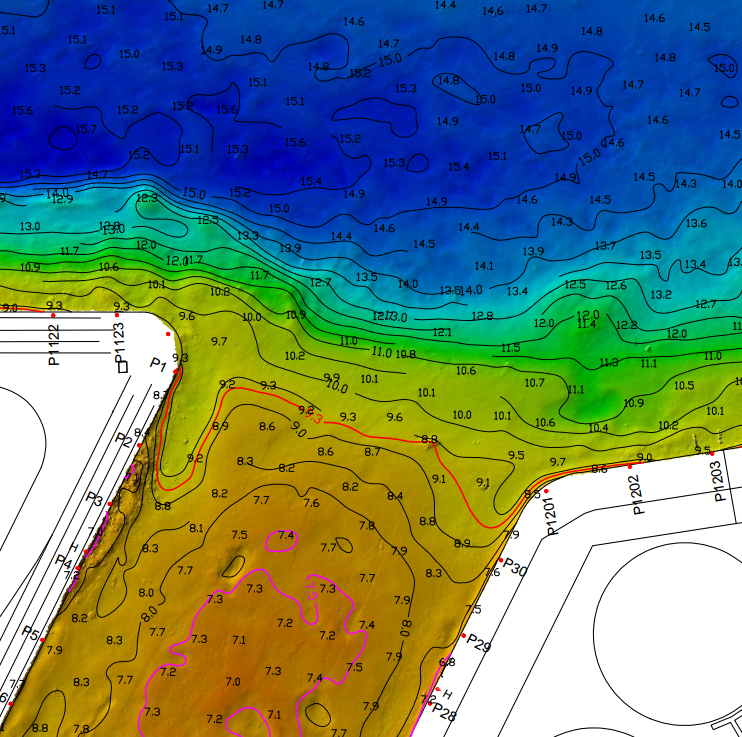
\includegraphics[width=.4\linewidth]{figures/smallDebthMapAalborg}
    \end{figure}
    \begin{itemize}
        \item Depth map used by Port of Aalborg 
        \item Problem: No recent knowledge of depths of the port
        \item Solution: Automate smaller unmanned vessel
    \end{itemize}
\end{frame}

\section{System Description}
\begin{frame}{System Description}{}
    \begin{minipage}{0.45\linewidth}
    \begin{figure}[H]
        \centering
        \includegraphics[width=1\linewidth]{figures/system}
    \end{figure}        
    \end{minipage}\hfill      
    \begin{minipage}{0.45\linewidth}
    \begin{figure}[H]
        \centering
        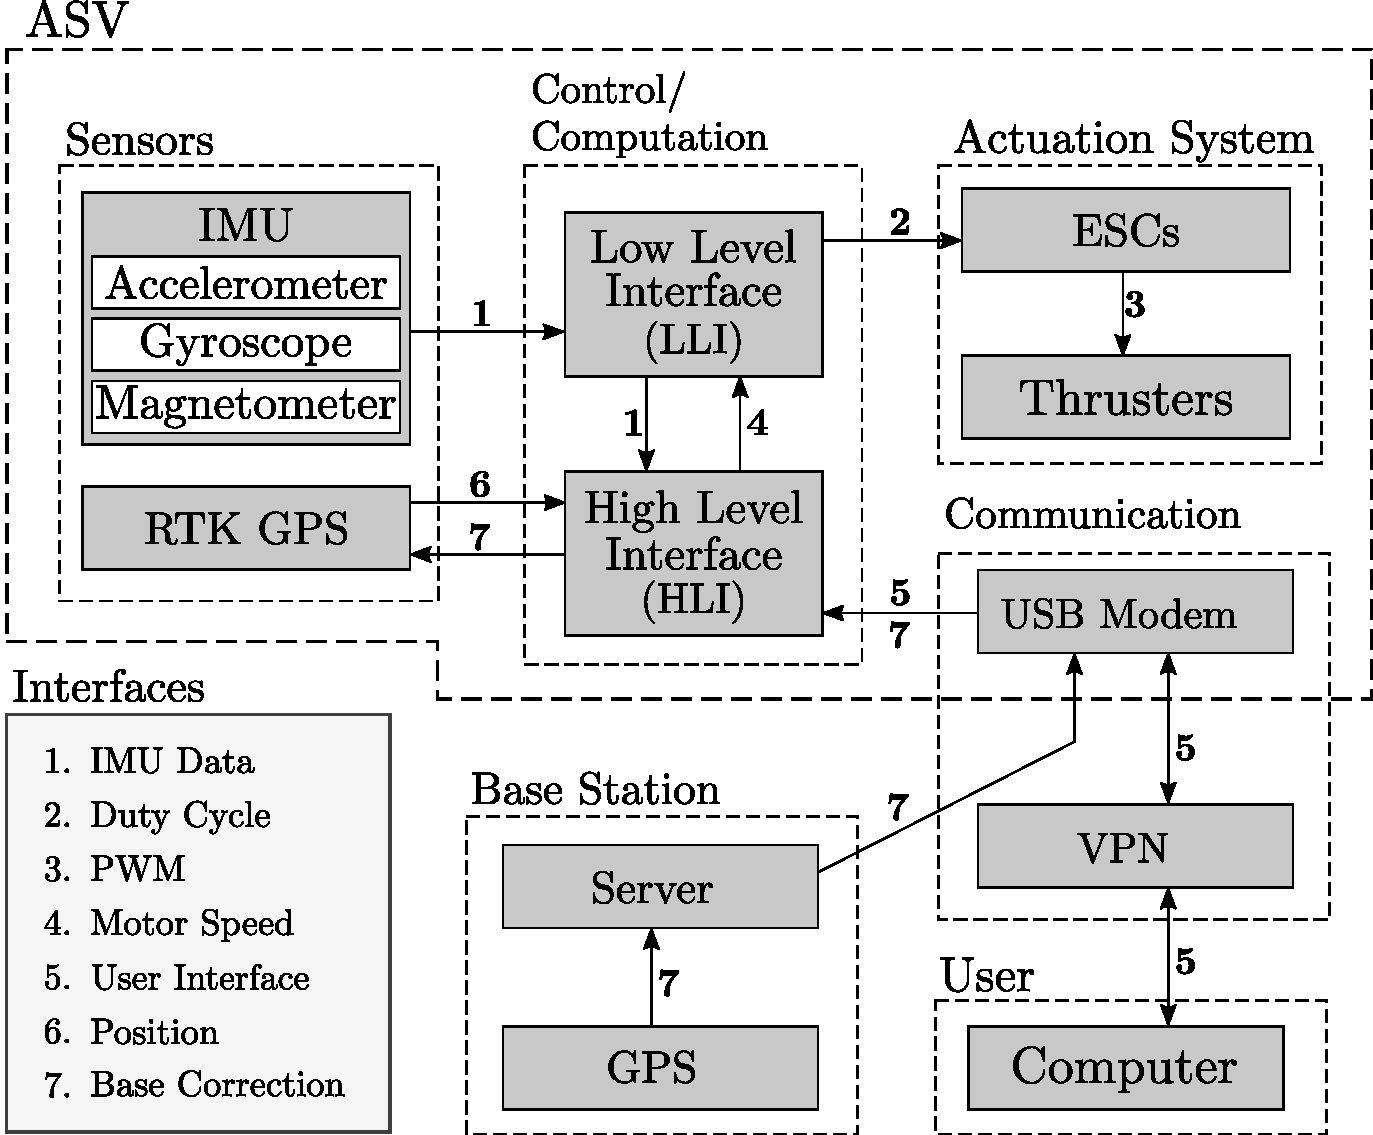
\includegraphics[width=1\linewidth]{figures/systemDiagram5}
    \end{figure}                
    \end{minipage}\hfill \\
\end{frame}

\begin{frame}{System Description}{RTK GPS}
    \begin{figure}[H]
        \centering
        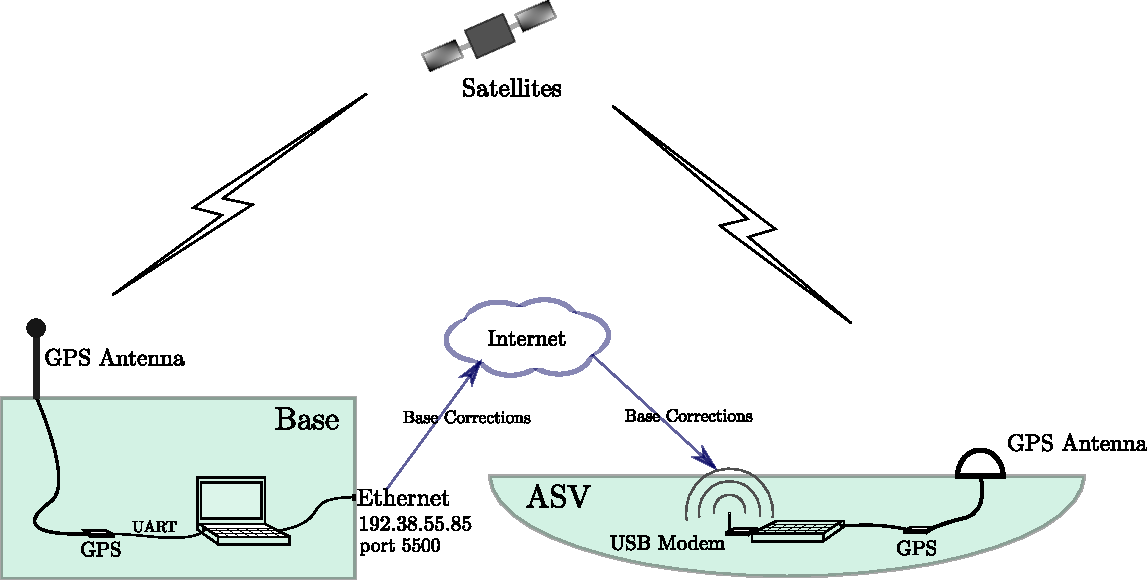
\includegraphics[width=0.7\linewidth]{figures/comunicationSetup}
    \end{figure}        

\end{frame}

%%%%%%%%%%%%%%%%
\section{Model}

%\subsection{Reference Frames}
\begin{frame}{Model}{Reference Frames}
    \begin{figure}[H]
        \centering
        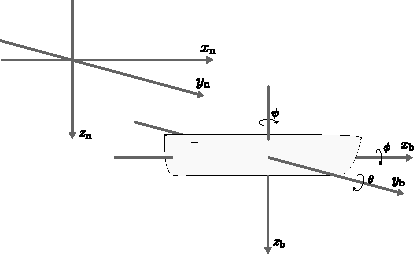
\includegraphics[width=0.7\linewidth]{figures/boat3D}
    \end{figure}
    \begin{itemize}
        \item Inertial Frame
        \item Body Frame
    \end{itemize}
\end{frame}

% %\subsection{Reference Frames}
% \begin{frame}{Model}{Reference Frames}
%     \begin{minipage}{0.65\linewidth}
%         \begin{figure}[H]
%             \centering
%             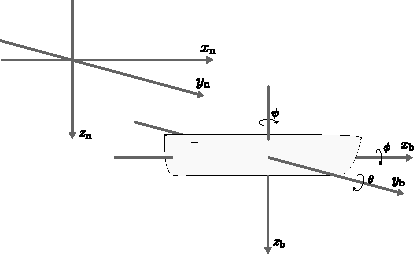
\includegraphics[width=1\linewidth]{figures/boat3D}
%         \end{figure}        
%     \end{minipage}\hfill      
%     \begin{minipage}{0.3\linewidth}
%         \begin{figure}[H]
%             \centering
%             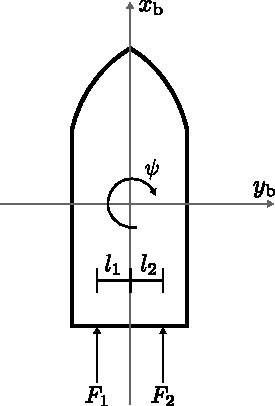
\includegraphics[width=0.7\linewidth]{figures/boat2D}
%         \end{figure}                
%     \end{minipage}\hfill \\
% \end{frame}

%\subsection{Model Dynamics}
\begin{frame}{Model}{Model Dynamics}
    \begin{minipage}{0.65\linewidth}
        \begin{figure}[H]
            \centering
            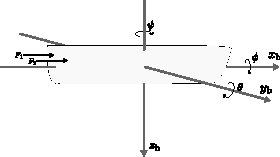
\includegraphics[width=1\linewidth]{figures/boat3DForces}
        \end{figure}        
    \end{minipage}\hfill      
    \begin{minipage}{0.3\linewidth}
        \begin{figure}[H]
            \centering
            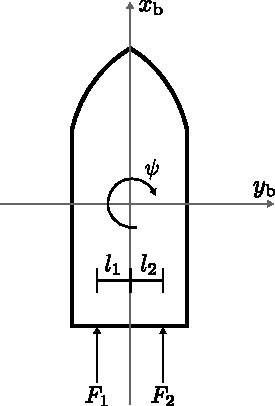
\includegraphics[width=0.7\linewidth]{figures/boat2D}
        \end{figure}                
    \end{minipage}\hfill \\
    \begin{itemize}
        \item Rigid Body Dynamics
        \item Hydrostatics
        \item Hydrodynamics
    \end{itemize}
\end{frame}

%\subsection{Rigid Body Dynamics}
\begin{frame}{Model}{Rigid Body Dynamics}
    \begin{minipage}{0.65\linewidth}
        \begin{figure}[H]
            \centering
            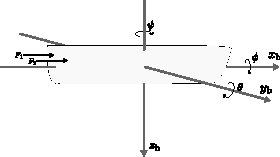
\includegraphics[width=1\linewidth]{figures/boat3DForces}
        \end{figure}        
    \end{minipage}\hfill      
    \begin{minipage}{0.3\linewidth}
        \begin{figure}[H]
            \centering
            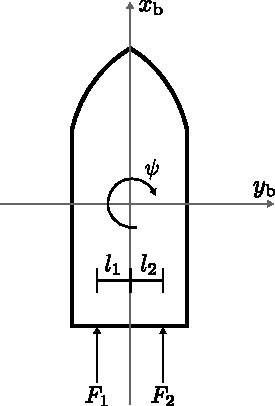
\includegraphics[width=0.7\linewidth]{figures/boat2D}
        \end{figure}                
    \end{minipage}\hfill \\
    \begin{flalign}
        \sum F&=m \ddot{x} \nonumber \\
        \sum \tau&=I \ddot{\theta} \nonumber
    \end{flalign}
\end{frame}

%\subsection{Hydrostatics}
\begin{frame}{Model}{Hydrostatics}
    \begin{minipage}{0.65\linewidth}
        \begin{figure}[H]
            \centering
            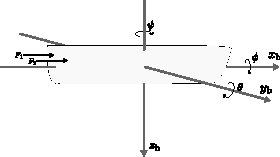
\includegraphics[width=1\linewidth]{figures/boat3DForces}
        \end{figure}        
    \end{minipage}\hfill      
    \begin{minipage}{0.3\linewidth}
        \begin{figure}[H]
            \centering
            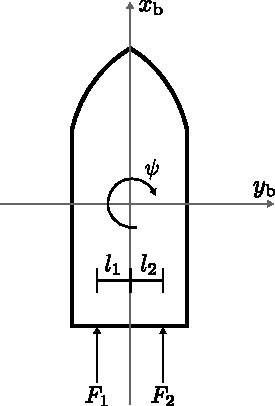
\includegraphics[width=0.7\linewidth]{figures/boat2D}
        \end{figure}                
    \end{minipage}\hfill \\
    \begin{itemize}
        \item Buoyancy Force
    \end{itemize}
\end{frame}

%\subsection{Hydrodynamics}
\begin{frame}{Model}{Hydrodynamics}
    \begin{minipage}{0.65\linewidth}
        \begin{figure}[H]
            \centering
            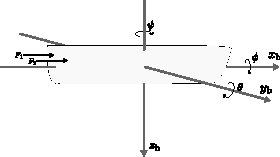
\includegraphics[width=1\linewidth]{figures/boat3DForces}
        \end{figure}        
    \end{minipage}\hfill      
    \begin{minipage}{0.3\linewidth}
        \begin{figure}[H]
            \centering
            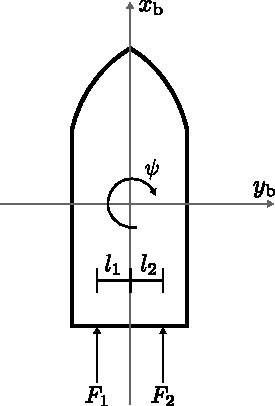
\includegraphics[width=0.7\linewidth]{figures/boat2D}
        \end{figure}                
    \end{minipage}\hfill \\
    \begin{itemize}
        \item Added mass
        \item Viscous Damping
    \end{itemize}
\end{frame}

%\subsection{Model Equations}
\begin{frame}{Model}{Model Equations}
    \begin{minipage}{0.5\linewidth}
        \begin{figure}[H]
            \centering
            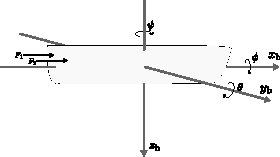
\includegraphics[width=1\linewidth]{figures/boat3DForces}
        \end{figure}        
    \end{minipage}\hfill      
    \begin{minipage}{0.5\linewidth}
        \begin{flalign}
            m \ddot{x}_\mathrm{b} &=  F_\mathrm{1} + F_\mathrm{2}  - d_{\dot{x}_\mathrm{b}} \dot{x}_\mathrm{b} + F_{x_\mathrm{b}}  \nonumber \\
            m \ddot{y}_\mathrm{b} &=  -d_{\dot{y}_\mathrm{b}} \dot{y_\mathrm{b}} + F_{y_\mathrm{b}}  \nonumber \\
            m \ddot{z}_\mathrm{b} &=  -d_{\dot{z}_\mathrm{b}}\dot{z_\mathrm{b}} + F_{z_\mathrm{b}}  \nonumber \\
            I_\mathrm{x}\ddot{\phi} &= -d_{\dot{\phi}} \dot{\phi} + T_\mathrm{\phi}   \nonumber \\
            I_\mathrm{y}\ddot{\theta} &= -d_{\dot{\theta}} \dot{\theta} + T_\mathrm{\theta}   \nonumber \\
            I_\mathrm{z}\ddot{\psi} &= F_\mathrm{1}l_\mathrm{1} - F_\mathrm{2} l_\mathrm{2} - d_{\dot{\psi}} \dot{\psi}  \nonumber
        \end{flalign}              
    \end{minipage}\hfill \\
\end{frame}

%\subsection{Model Equations}
\begin{frame}{Model}{Linearized Model Equations}
    \begin{minipage}{0.5\linewidth}
        \begin{figure}[H]
            \centering
            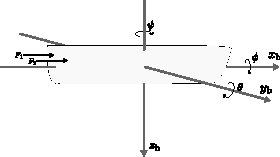
\includegraphics[width=1\linewidth]{figures/boat3DForces}
        \end{figure}        
    \end{minipage}\hfill      
    \begin{minipage}{0.5\linewidth}
        \begin{flalign}
            m \ddot{x}_\mathrm{b} &=  F_\mathrm{1} + F_\mathrm{2}  - d_{\dot{x}_\mathrm{b}} \dot{x}_\mathrm{b} \nonumber \\
            m \ddot{y}_\mathrm{b} &=  -d_{\dot{y}_\mathrm{b}} \dot{y_\mathrm{b}} \nonumber \\
            m \ddot{z}_\mathrm{b} &=  -d_{\dot{z}_\mathrm{b}}\dot{z_\mathrm{b}} -\rho g A_\mathrm{wp} \tilde{z}_\mathrm{n} \nonumber  \\
            I_\mathrm{x}\ddot{\phi} &= -d_{\dot{\phi}} \dot{\phi} - \rho g V \overline{GM_{T}}\cdot \phi \nonumber \\
            I_\mathrm{y}\ddot{\theta} &= -d_{\dot{\theta}} \dot{\theta} - \rho g V \overline{GM_{L}}\cdot \theta \nonumber \\
            I_\mathrm{z}\ddot{\psi} &= F_\mathrm{1}l_\mathrm{1} - F_\mathrm{2} l_\mathrm{2} - d_{\dot{\psi}} \dot{\psi} \nonumber
        \end{flalign}              
    \end{minipage}\hfill \\
\end{frame}

% %\subsection{Model Equations 2}
% \begin{frame}{Model}{Model Equations 2}
%     \begin{minipage}{0.3\linewidth}
%         \begin{figure}[H]
%             \centering
%             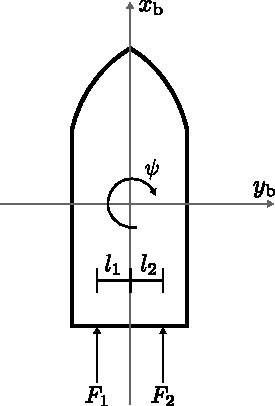
\includegraphics[width=1\linewidth]{figures/boat2D}
%         \end{figure}        
%     \end{minipage}\hfill      
%     \begin{minipage}{0.65\linewidth}
%         \begin{flalign}
%             m \ddot{x}_\mathrm{b} &=  F_\mathrm{1} + F_\mathrm{2}  - d_{\dot{x}_\mathrm{b}} \dot{x}_\mathrm{b} + F_{x_\mathrm{b}}  \nonumber \\
%             m \ddot{y}_\mathrm{b} &=  -d_{\dot{y}_\mathrm{b}} \dot{y_\mathrm{b}} + F_{y_\mathrm{b}}  \nonumber \\
%             m \ddot{z}_\mathrm{b} &=  -d_{\dot{z}_\mathrm{b}}\dot{z_\mathrm{b}} + F_{z_\mathrm{b}}  \nonumber \\
%             I_\mathrm{x}\ddot{\phi} &= -d_{\dot{\phi}} \dot{\phi} + T_\mathrm{\phi}   \nonumber \\
%             I_\mathrm{y}\ddot{\theta} &= -d_{\dot{\theta}} \dot{\theta} + T_\mathrm{\theta}   \nonumber \\
%             I_\mathrm{z}\ddot{\psi} &= F_\mathrm{1}l_\mathrm{1} - F_\mathrm{2} l_\mathrm{2} - d_{\dot{\psi}} \dot{\psi}  \nonumber
%         \end{flalign}              
%     \end{minipage}\hfill \\
% \end{frame}

%\subsection{Model Verification}
\begin{frame}{Model}{Model Verification}
    \begin{itemize}
        \item Verified Nonlinear Model
    \end{itemize}
    \begin{minipage}{0.45\linewidth}
        \begin{figure}[H]
            \centering
            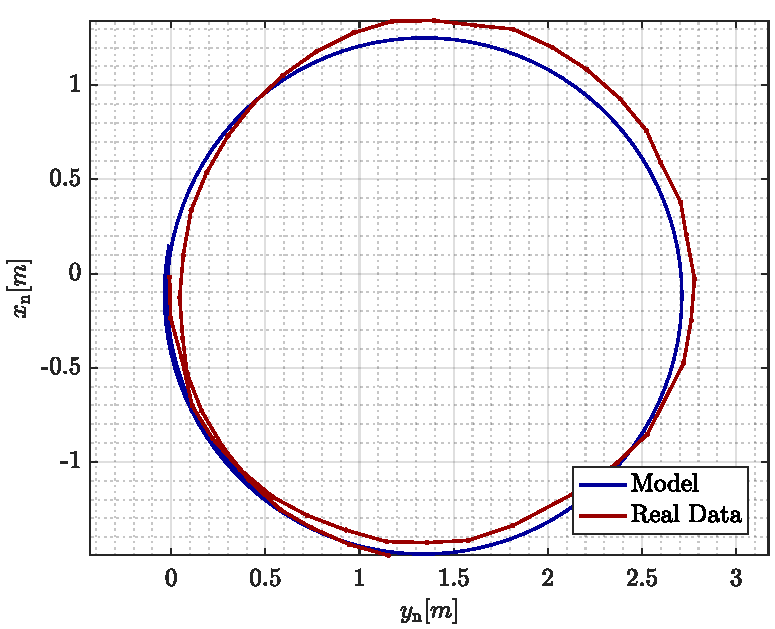
\includegraphics[width=1\linewidth]{figures/turn}
        \end{figure}        
    \end{minipage}\hfill      
    \begin{minipage}{0.45\linewidth}
        \begin{figure}[H]
            \centering
            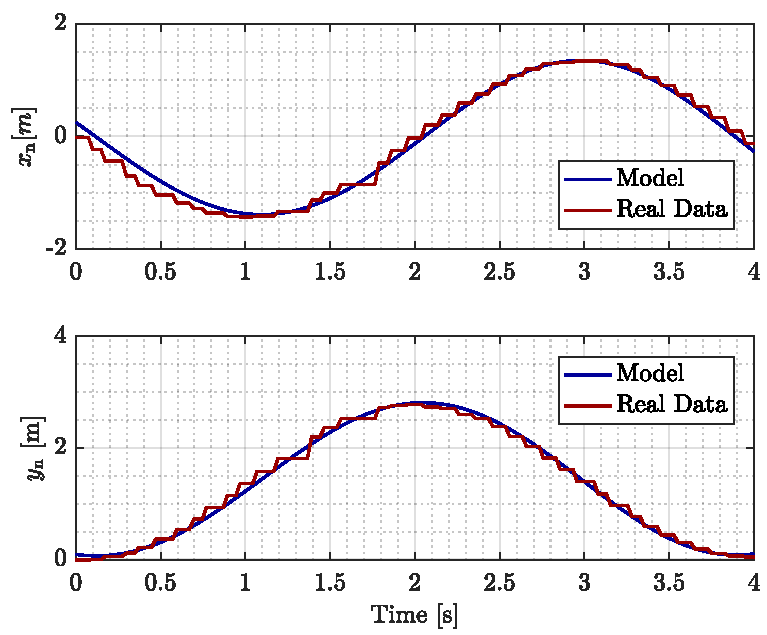
\includegraphics[width=1\linewidth]{figures/turn_time}
        \end{figure}                
    \end{minipage}\hfill \\
\end{frame}








\definecolor{aaublue}{RGB}{33,26,82}% dark blue

\begin{frame}{Agenda}{}
    \begin{itemize}
        \item Introduction
        \item System Description
        \item Model
        \item \textcolor{aaublue}{\textbf{Control Approach}}
        \item \textcolor{aaublue}{\textbf{Sensor Fusion}}
        \begin{itemize}
            \item[-] \textcolor{aaublue}{\textbf{Attitude Kalman Filter}}
            \item[-] \textcolor{aaublue}{\textbf{Position Kalman Filter}}
        \end{itemize}
        \item Inner Controller
        \item Outer Controller
        \item Results
        \item Conclusion
    \end{itemize}
\end{frame}
%%%%%%%%%%%%%%%%
\section{Control Approach}

\begin{frame}{Control Approach}{}
    \begin{figure}[H]
        \centering
        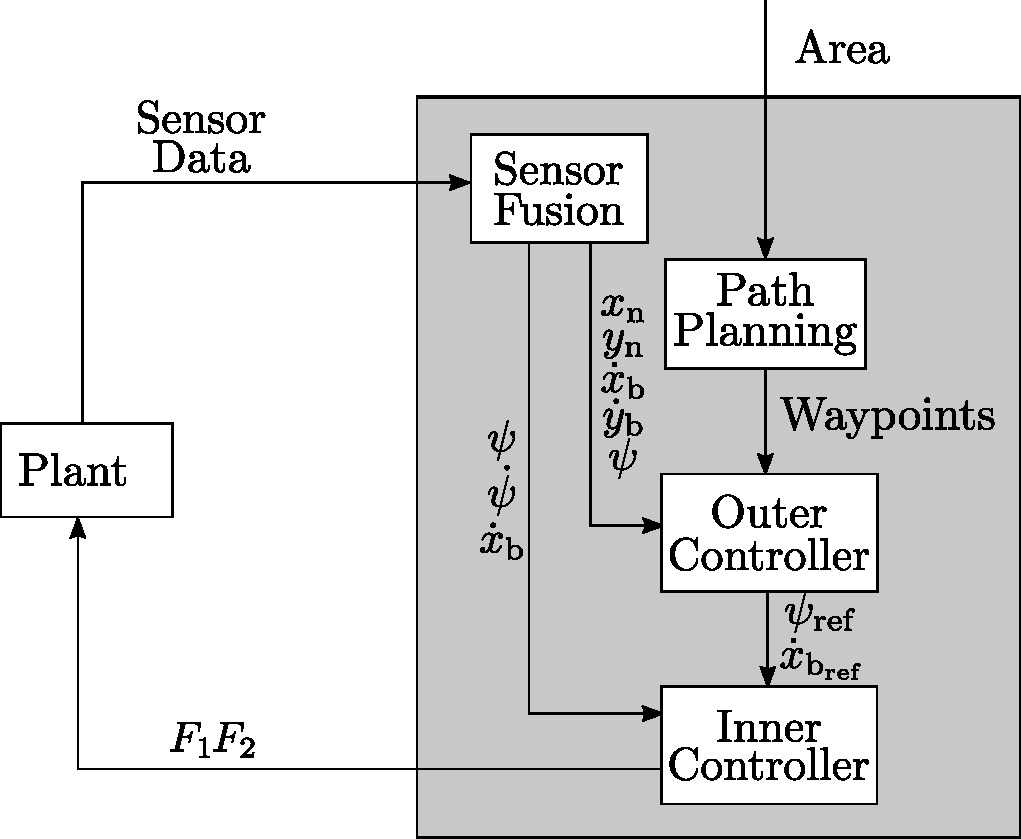
\includegraphics[width=.6\linewidth]{figures/controllerDiagram2}
    \end{figure}
\end{frame}

%%%%%%%%%%%%%%%%
\section{Sensor Fusion}

\begin{frame}{Sensor Fusion}{Structure}
	\begin{itemize}

		\item Fuses GPS and IMU data
		\item Achieved using a Kalman filter
		\item Sensor fusion contains
			\begin{itemize}
		\item Attitude
		\item Position
			\end{itemize}
	\end{itemize}

\end{frame}
\begin{frame}{Sensor Fusion}{Signal Model}
	\begin{gather*}
    \vec{x}_\mathrm{KF}(k+1) = \vec{A}\vec{x}_\mathrm{KF}(k) + \vec{B}_\mathrm{KF} \vec{u}(k) + \vec{w}_\mathrm{KF}(k)  \nonumber \\
    \vec{y}_\mathrm{KF}(k) = \vec{C}_\mathrm{KF} \vec{x}_\mathrm{KF}(k) + \vec{v}_\mathrm{KF}(k)  \nonumber
    \end{gather*}
    \begin{figure}[H]
        \centering
        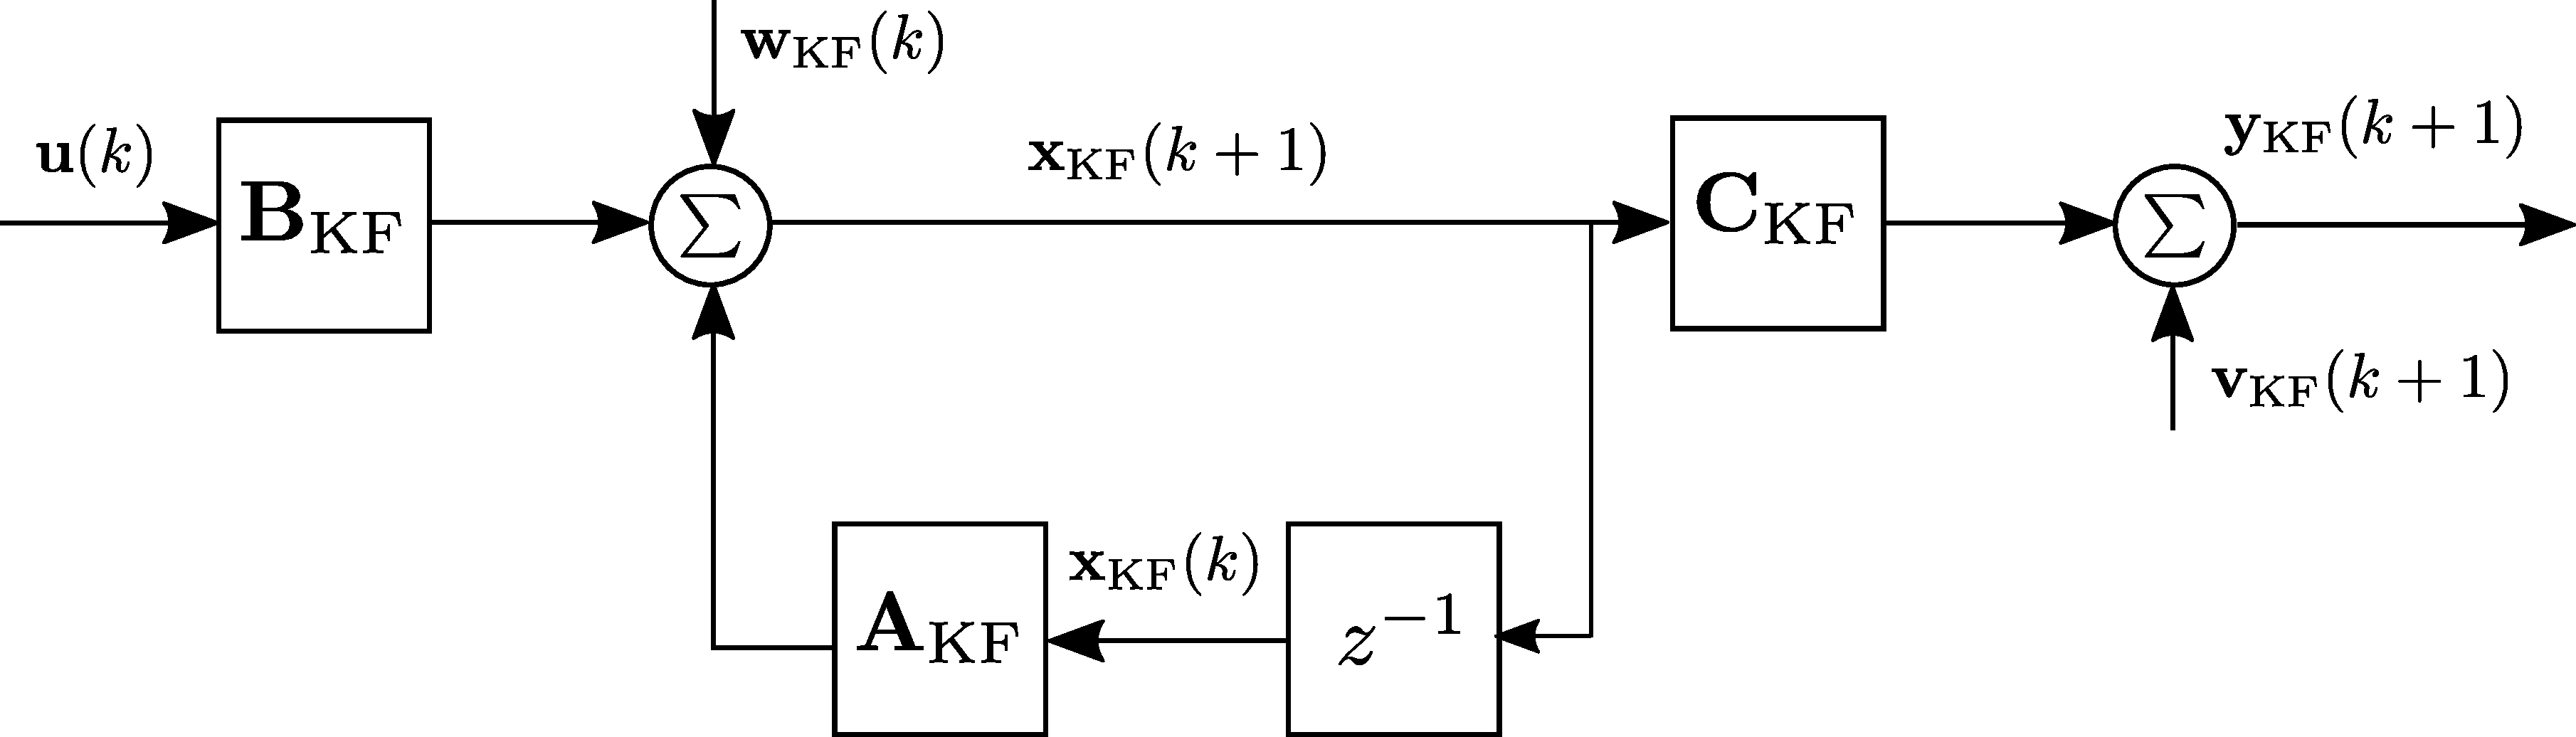
\includegraphics[width=.7\linewidth]{figures/signalModel}
    \end{figure}

	\begin{itemize}
		\item w(k) and v(k) are assumed white Gaussian
		\item Matrices $\vec{Q}_\mathrm{KF}$ and $\vec{R}_\mathrm{KF}$ contain the respective covariances
	\end{itemize}

\end{frame}

\begin{frame}{Sensor Fusion}{Signal Model - State and Measurement Vectors}
\begin{itemize}
    \item Attitude
    \begin{gather*}
        \vec{x}_\mathrm{att} = 
        \begin{bmatrix}
        \phi & \theta & \psi & \dot{\phi} & \dot{\theta} & \dot{\psi} & \ddot{\phi} & \ddot{\theta} & \ddot{\psi}
        \end{bmatrix}^\mathrm{T}  \nonumber \\
        \vec{y}_\mathrm{att} =
        \begin{bmatrix}
        \phi_\mathrm{acc} & \theta_\mathrm{acc} & \psi_\mathrm{mag} & \dot{\phi}_\mathrm{gyro} & \dot{\theta}_\mathrm{gyro} & \dot{\psi}_\mathrm{gyro}
        \end{bmatrix}^\mathrm{T} \nonumber
    \end{gather*}
	\item Position
    \begin{gather*}
        \vec{x}_\mathrm{pos} =
        \begin{bmatrix}
        x_\mathrm{n} & y_\mathrm{n} & \dot{x}_\mathrm{b} & \dot{y}_\mathrm{b} & \ddot{x}_\mathrm{b} & \ddot{y}_\mathrm{b}
        \end{bmatrix}^\mathrm{T} \nonumber \\
        \vec{y}_\mathrm{pos} =
        \begin{bmatrix}
        x_\mathrm{n,GPS} & y_\mathrm{n,GPS} & \ddot{x}_\mathrm{b,acc} & \ddot{y}_\mathrm{b,acc}
        \end{bmatrix}^\mathrm{T} \nonumber
    \end{gather*}
    \end{itemize}
\end{frame}


\begin{frame}{Sensor Fusion}{Kalman Filter}

	\begin{itemize}
		\item Step 0: Initialization
        \begin{flalign}
        	\hat{\vec{x}}_\mathrm{KF}(0|0) &= \vec{0} \nonumber\\
        	\vec{P}_\mathrm{KF}(0|0) &= \vec{Q}_\mathrm{KF}\nonumber
        \end{flalign}
		\item Step 1: Prediction
		\item Step 2: Update
   	\end{itemize}
\end{frame}


\begin{frame}{Sensor Fusion}{Kalman Filter}
	\begin{itemize}
		\item Step 0: Initialization
		\item Step 1: Prediction
        {\footnotesize
        \begin{flalign}
            \hat{\vec{x}}_\mathrm{KF}(k+1|k) &= \vec{A}_\mathrm{KF} \hat{\vec{x}}_\mathrm{KF}(k|k) + \vec{B}_\mathrm{KF} \vec{u}(k) \nonumber\\
            \vec{P}(k+1|k) &= \vec{A}_\mathrm{KF} \vec{P}(k|k) \vec{A}_\mathrm{KF}^\mathrm{T} + \vec{Q}_\mathrm{KF} \nonumber
        \end{flalign}}
	 	\item Step 2: Update
         {\footnotesize
        \begin{gather*}
            \hat{\vec{x}}_\mathrm{KF}(k+1|k+1) = \hat{\vec{x}}_\mathrm{KF}(k+1|k) +  \vec{K}(k+1) \left[ \vec{y}_\mathrm{KF}(k+1) - \vec{C}_\mathrm{KF}  \hat{\vec{x}}_\mathrm{KF}(k+1|k) \right] \nonumber\\
            \vec{P}(k+1|k+1) = \left[ \vec{I} - \vec{K}(k+1) \vec{C}_\mathrm{KF}^\mathrm{T} \right] \vec{P}(k+1|k)\nonumber\\
        	\vec{K}(k+1) =  \vec{P}(k+1|k) \vec{C}_\mathrm{KF}^\mathrm{T}  \left[\vec{C}_\mathrm{KF} \vec{P}(k+1|k) \vec{C}_\mathrm{KF}^\mathrm{T} + \vec{R}_\mathrm{KF} \right]^{-1}\nonumber 
        \end{gather*}}
	\end{itemize}
\end{frame}

\begin{frame}{Sensor Fusion}{Kalman Filter}
    \begin{figure}[H]
        \centering
        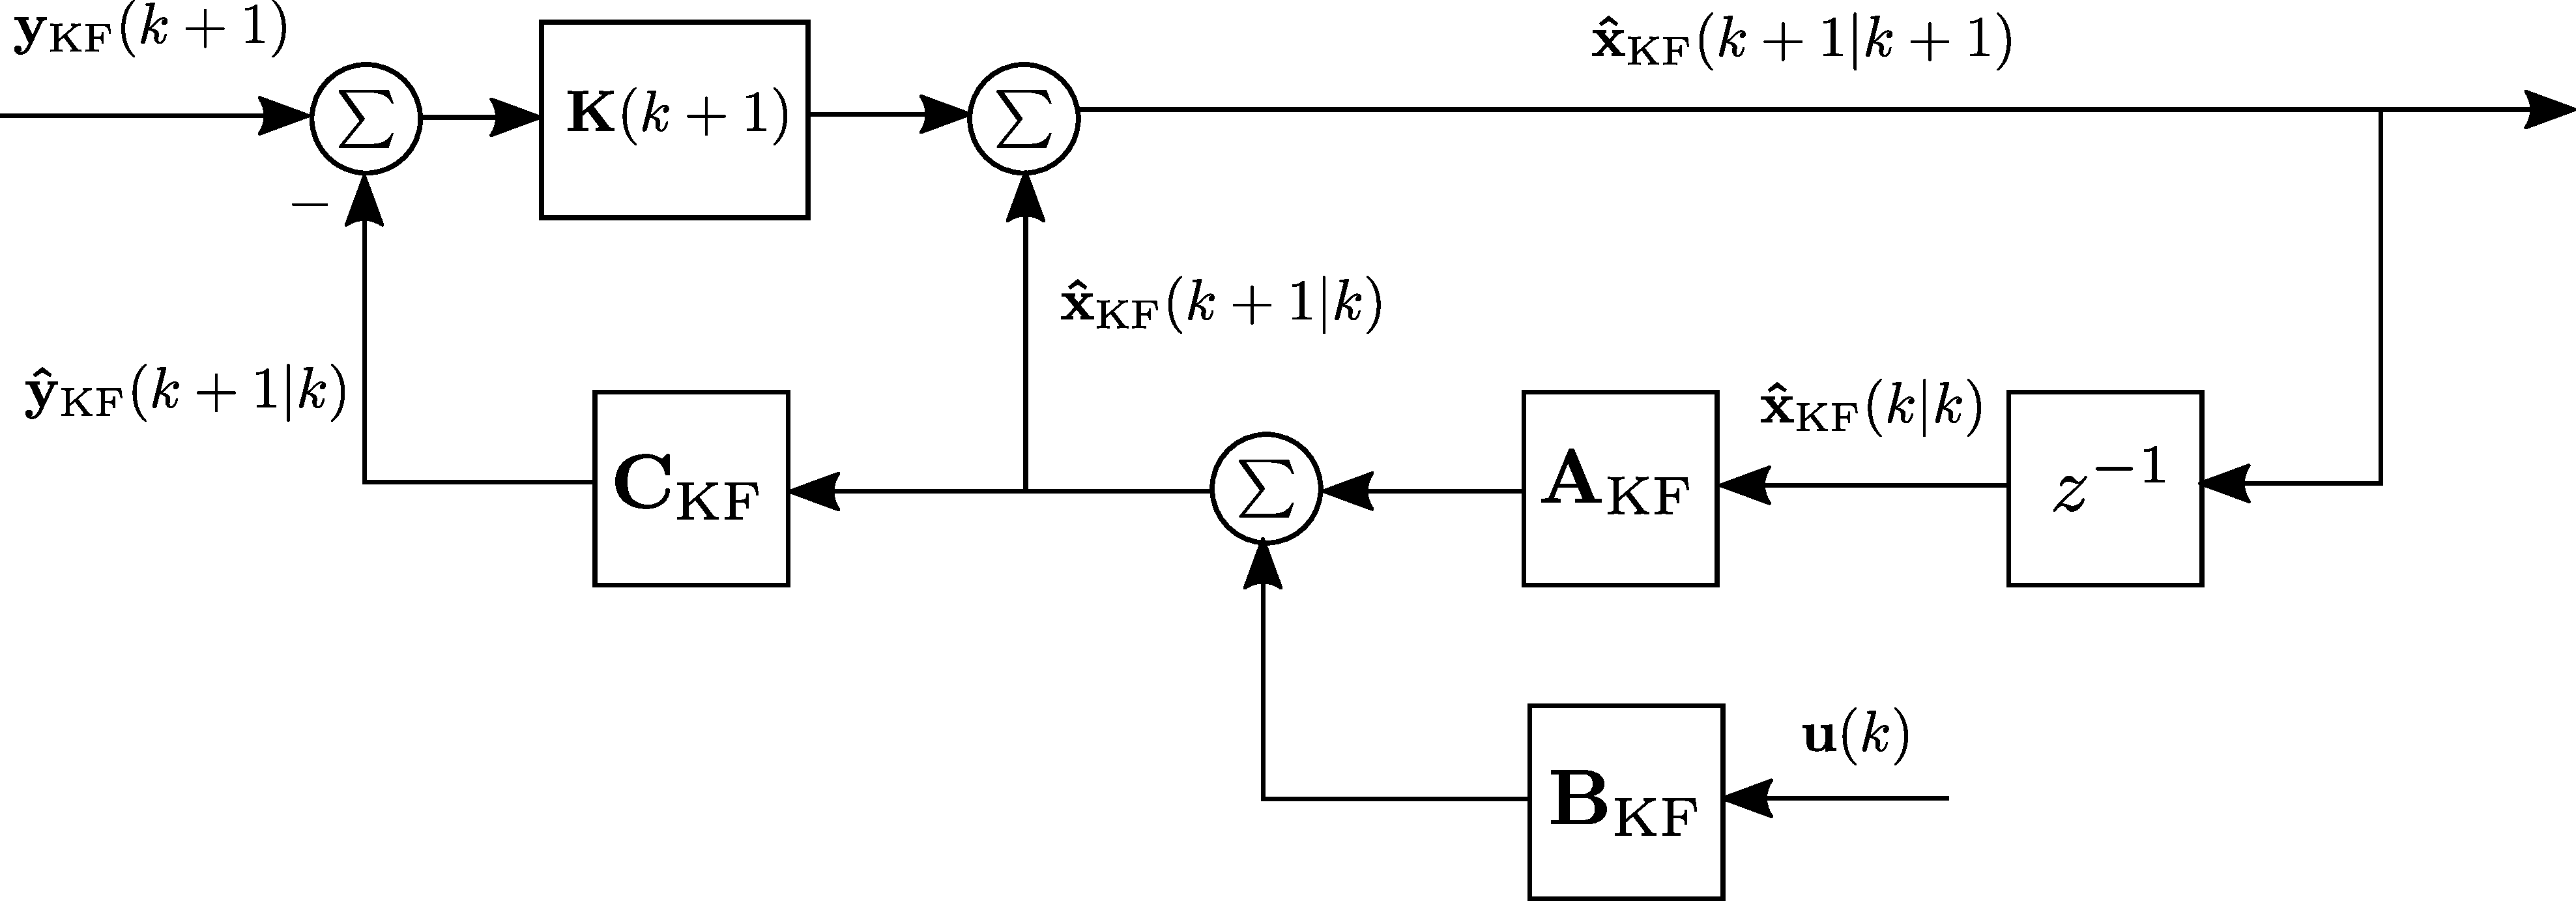
\includegraphics[width=.95\linewidth]{figures/kalmanFilter}
    \end{figure}
\end{frame}

\begin{frame}{Sensor Fusion}{Attitude Kalman Filter}
    \begin{figure}[H]
        \centering
        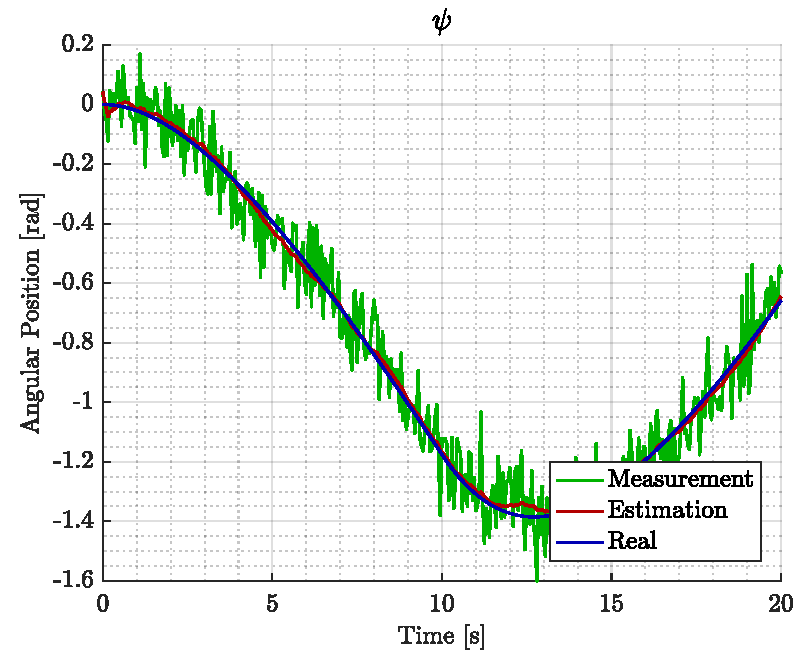
\includegraphics[width=0.6\linewidth]{figures/sim_yaw}
    \end{figure}
\end{frame}

\begin{frame}{Sensor Fusion}{Position Kalman Filter}
    \begin{minipage}{0.45\linewidth}
        \begin{figure}[H]
            \centering
            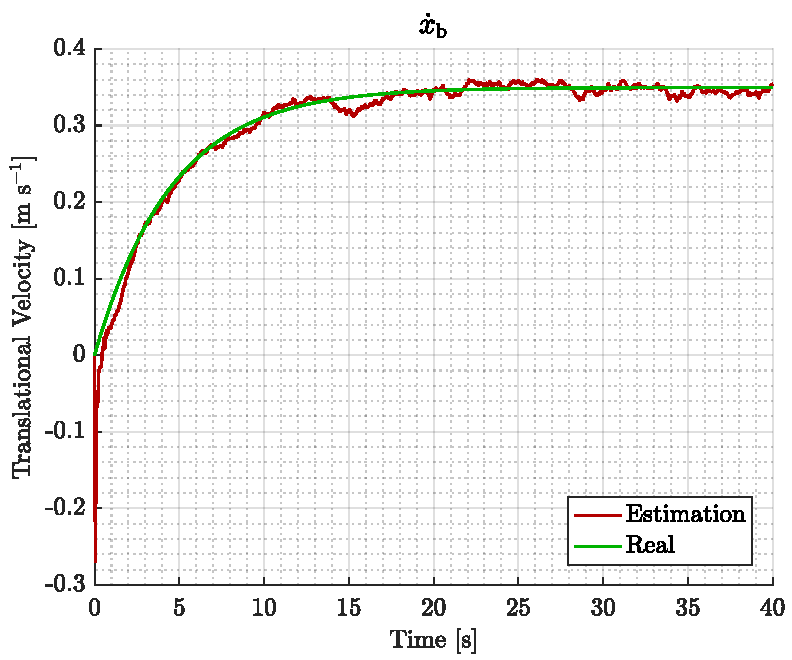
\includegraphics[width=1\linewidth]{figures/sim_xbdot}
        \end{figure}        
    \end{minipage}\hfill      
    \begin{minipage}{0.45\linewidth}
        \begin{figure}[H]
            \centering
            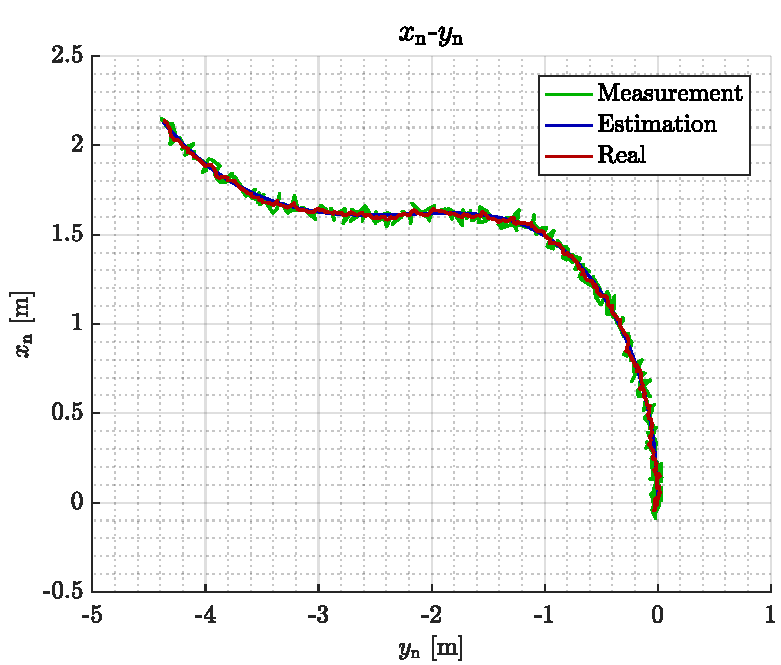
\includegraphics[width=1\linewidth]{figures/sim_xnyn}
        \end{figure}                
    \end{minipage}\hfill \\
\end{frame}



\begin{frame}{Agenda}{}
    \begin{itemize}
        \item Introduction
        \item System Description
        \item Model
        \item Control Approach
        \item Sensor Fusion
        \item \textbf{Inner Controller}
        \begin{itemize}
            \item[-] \textbf{Robust Controller Design}
            \item[-] Linear Quadratic Regulator Design
            \item[-] Comparison of the Controllers
        \end{itemize}
        \item Outer Controller
        \item Results
        \item Conclusion
    \end{itemize}
\end{frame}
%%%%%%%%%%%%%%%%
\section{Inner Controller}

\begin{frame}{Inner Controller}{}
    \uncover<1-2>{
    \begin{figure}[H]
        \centering
        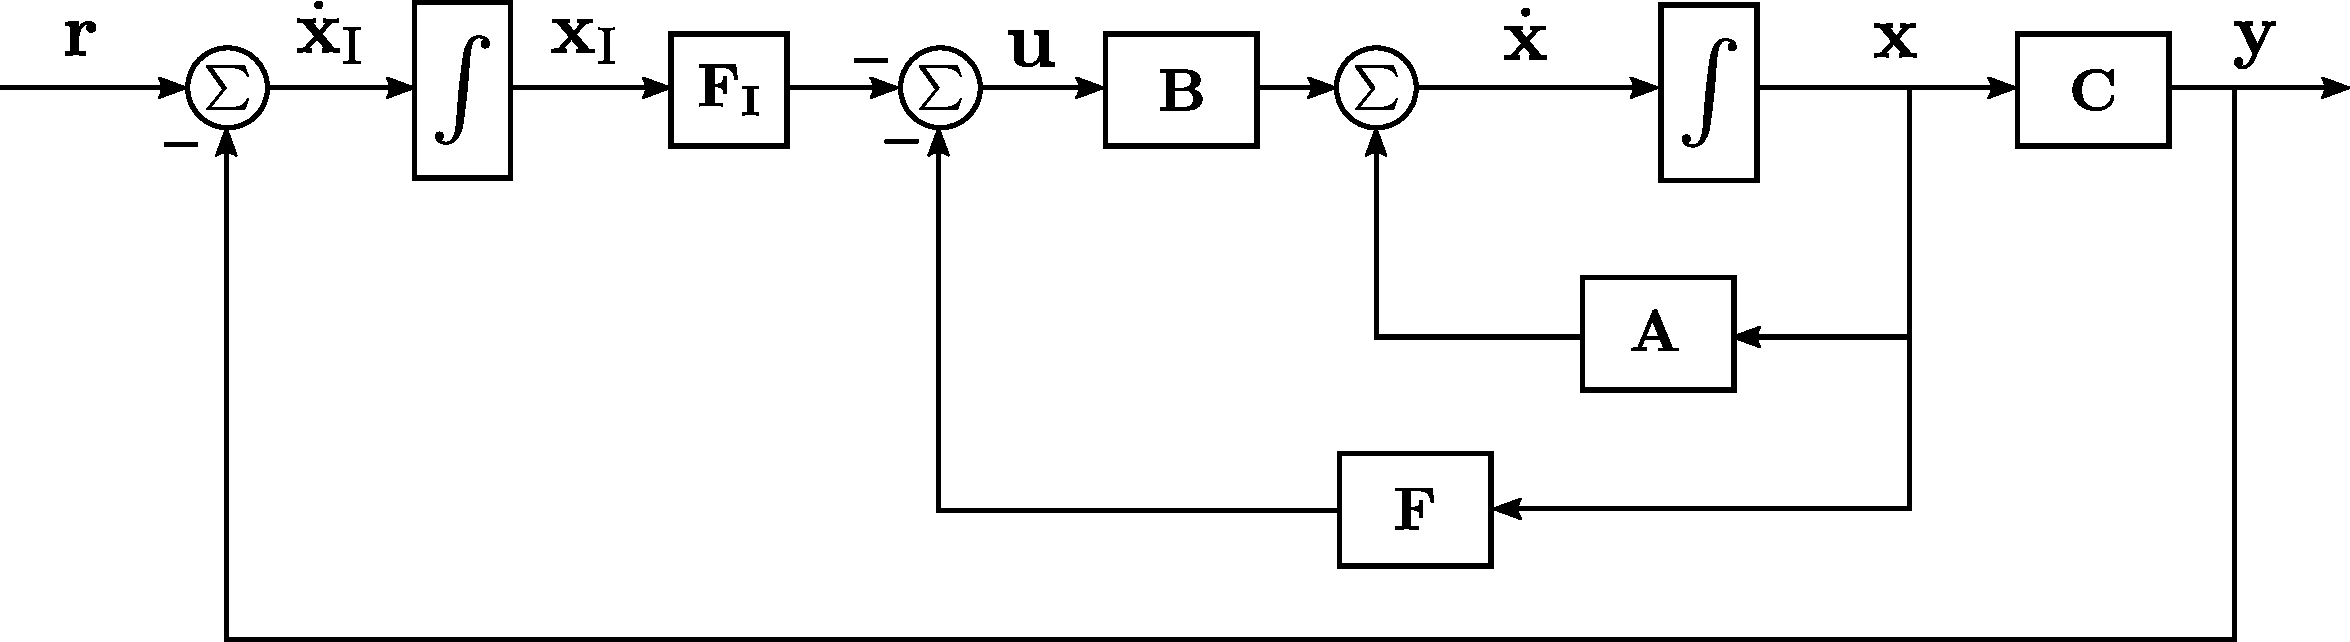
\includegraphics[width=1\linewidth]{figures/HinfControlBlockDiagram}
    \end{figure}}
    \uncover<2>{
    \begin{itemize}
        \item $\mathcal{H}_\infty$ Controller
        \item Linear Quadratic Regulator
    \end{itemize}}
\end{frame}

\begin{frame}{Inner Controller}{$\mathcal{H}_\infty$ Controller Design}
    \begin{itemize}
        \item Suboptimal $\mathcal{H}_\infty$ controller
    \end{itemize}
    \vspace{0.2cm}
    \begin{center}
        Find an internally stabilizing controller that provides a closed loop $\mathcal{H}_\infty$ norm less than some bound $\gamma$
    \end{center}
\end{frame}

\begin{frame}{Inner Controller}{$\mathcal{H}_\infty$ Controller Design}
    \begin{itemize}
        \item System structure
    \end{itemize}
    \begin{figure}[H]
        \centering
        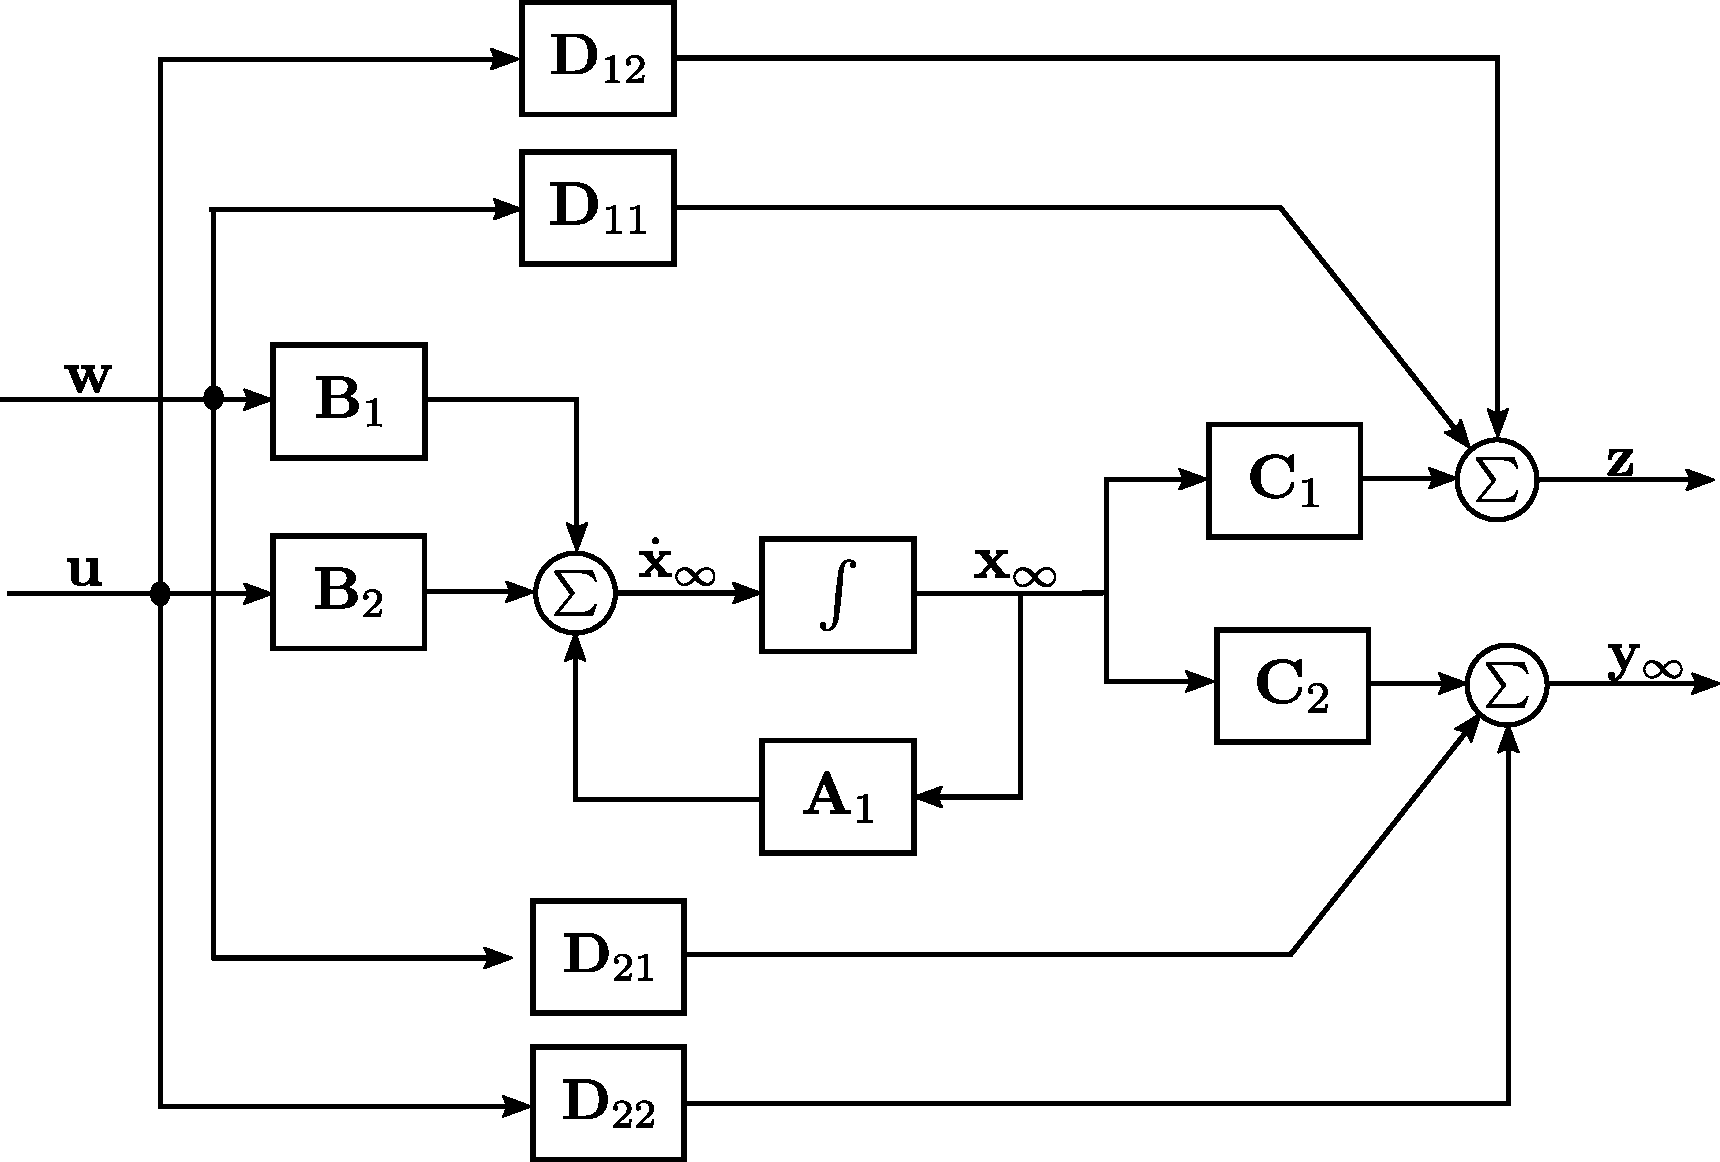
\includegraphics[width=0.55\linewidth]{figures/HinfDiag}
    \end{figure}
    \begin{minipage}[c][2.5cm]{\textwidth}
    \only<1|handout:1>{
    \begin{flalign}
    	\dot{\vec{x}}_\infty(t) &= \vec{A}_1 \vec{x}_\infty(t) + \vec{B}_1 \vec{w}(t) + \vec{B}_2 \vec{u}(t)\nonumber\\
    	\vec{z}(t) &= \vec{C}_1 \vec{x}_\infty(t) + \vec{D}_{11} \vec{w}(t) + \vec{D}_{12} \vec{u}(t)\nonumber\\
    	\vec{y}_\infty(t) &= \vec{C}_2 \vec{x}_\infty(t) + \vec{D}_{21} \vec{w}(t) + \vec{D}_{22} \vec{u}(t)\nonumber
    \end{flalign}}
    \only<2|handout:0>{
    \begin{flalign}	
    	\vec{u}(t) &= 
    	\begin{bmatrix}
    	F_1 & F_2 
    	\end{bmatrix}^\mathrm{T}\nonumber 
    \end{flalign}}
    \only<3|handout:0>{
    \begin{flalign}	
    	\vec{w}(t) &= 
    	\begin{bmatrix}
    	\psi_\mathrm{ref} & \dot{x}_\mathrm{b,ref} & F_\mathrm{wc} & \tau_\mathrm{wc} & F_\mathrm{wave} & \tau_\mathrm{wave}& n_{\psi} & n_{\dot{x}_\mathrm{b}}
    	\end{bmatrix}^\mathrm{T} \nonumber 
    \end{flalign}}
    \only<4|handout:0>{
    \begin{flalign}
    	\vec{y}_\infty(t) &= 
    	\begin{bmatrix}
    	\psi & \dot{x}_\mathrm{b} & \vec{x}_\mathrm{I}^\mathrm{T}
    	\end{bmatrix}^\mathrm{T}\nonumber 
    \end{flalign}}
    \only<5|handout:0>{
        \vspace{-0.55cm}
        \begin{flalign}
        \vec{x}_\infty(t) &=
        \begin{bmatrix}
        \psi & \dot{\psi} & \dot{x}_\mathrm{b} & x_{I_{\psi}} & x_{I_{\dot{x}_\mathrm{b}}} & x_{F_\mathrm{wc}} & x_{\tau_\mathrm{wc}} & x_{F_\mathrm{wave}} & x_{\tau_\mathrm{wave}} & x_{n_{\psi}}\ \ \  x_{n_{\dot{x}_\mathrm{b}}}
        \end{bmatrix}^\mathrm{T} \nonumber 
        \end{flalign}}
    \end{minipage}
\end{frame}

\begin{frame}{Inner Controller}{$\mathcal{H}_\infty$ Controller Design}
    \begin{itemize}
        \item Disturbance model
    \end{itemize}  
    \begin{figure}[H]
        \centering
        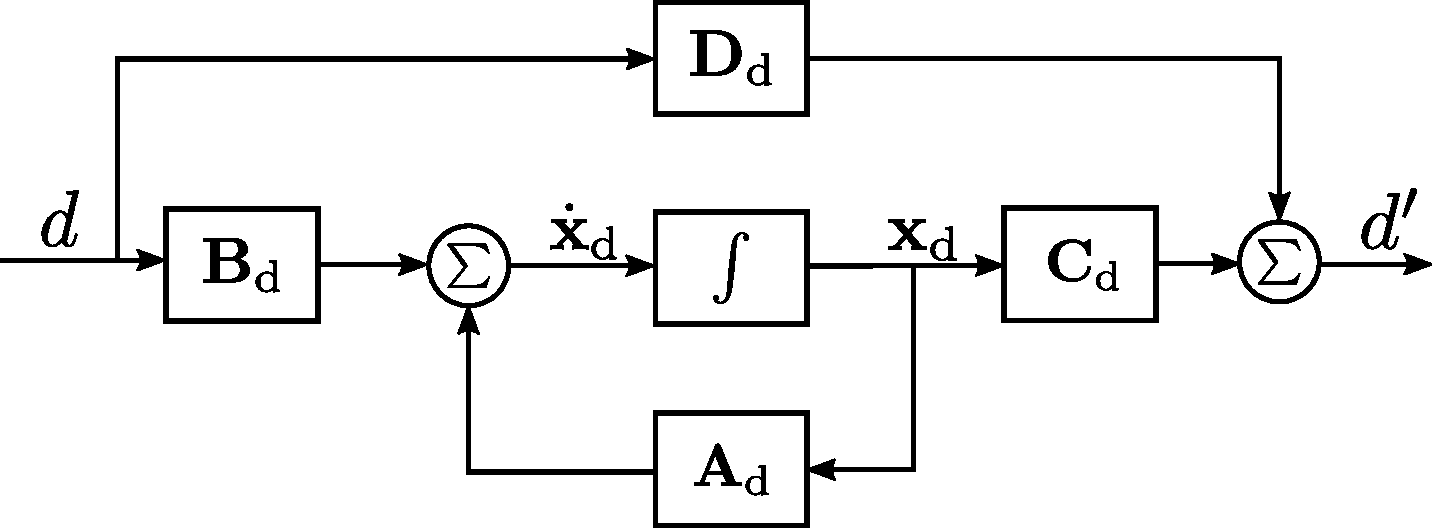
\includegraphics[width=0.6\linewidth]{figures/WeightDiag}
      \end{figure} 
      \begin{flalign}
      \frac{d'}{d}=\frac{a}{s+a} \rightarrow \dot{d}' = -a d' + a d \rightarrow \begin{cases} \dot{x}_\mathrm{d} = -a x_\mathrm{d} + a d \\ d' = x_\mathrm{d} \end{cases} \nonumber
      \end{flalign}    
\end{frame}
 
    
\begin{frame}<handout:0>{Inner Controller}{$\mathcal{H}_\infty$ Controller Design}
    \begin{itemize}
        \item System structure
    \end{itemize}
    \begin{figure}[H]
        \centering
        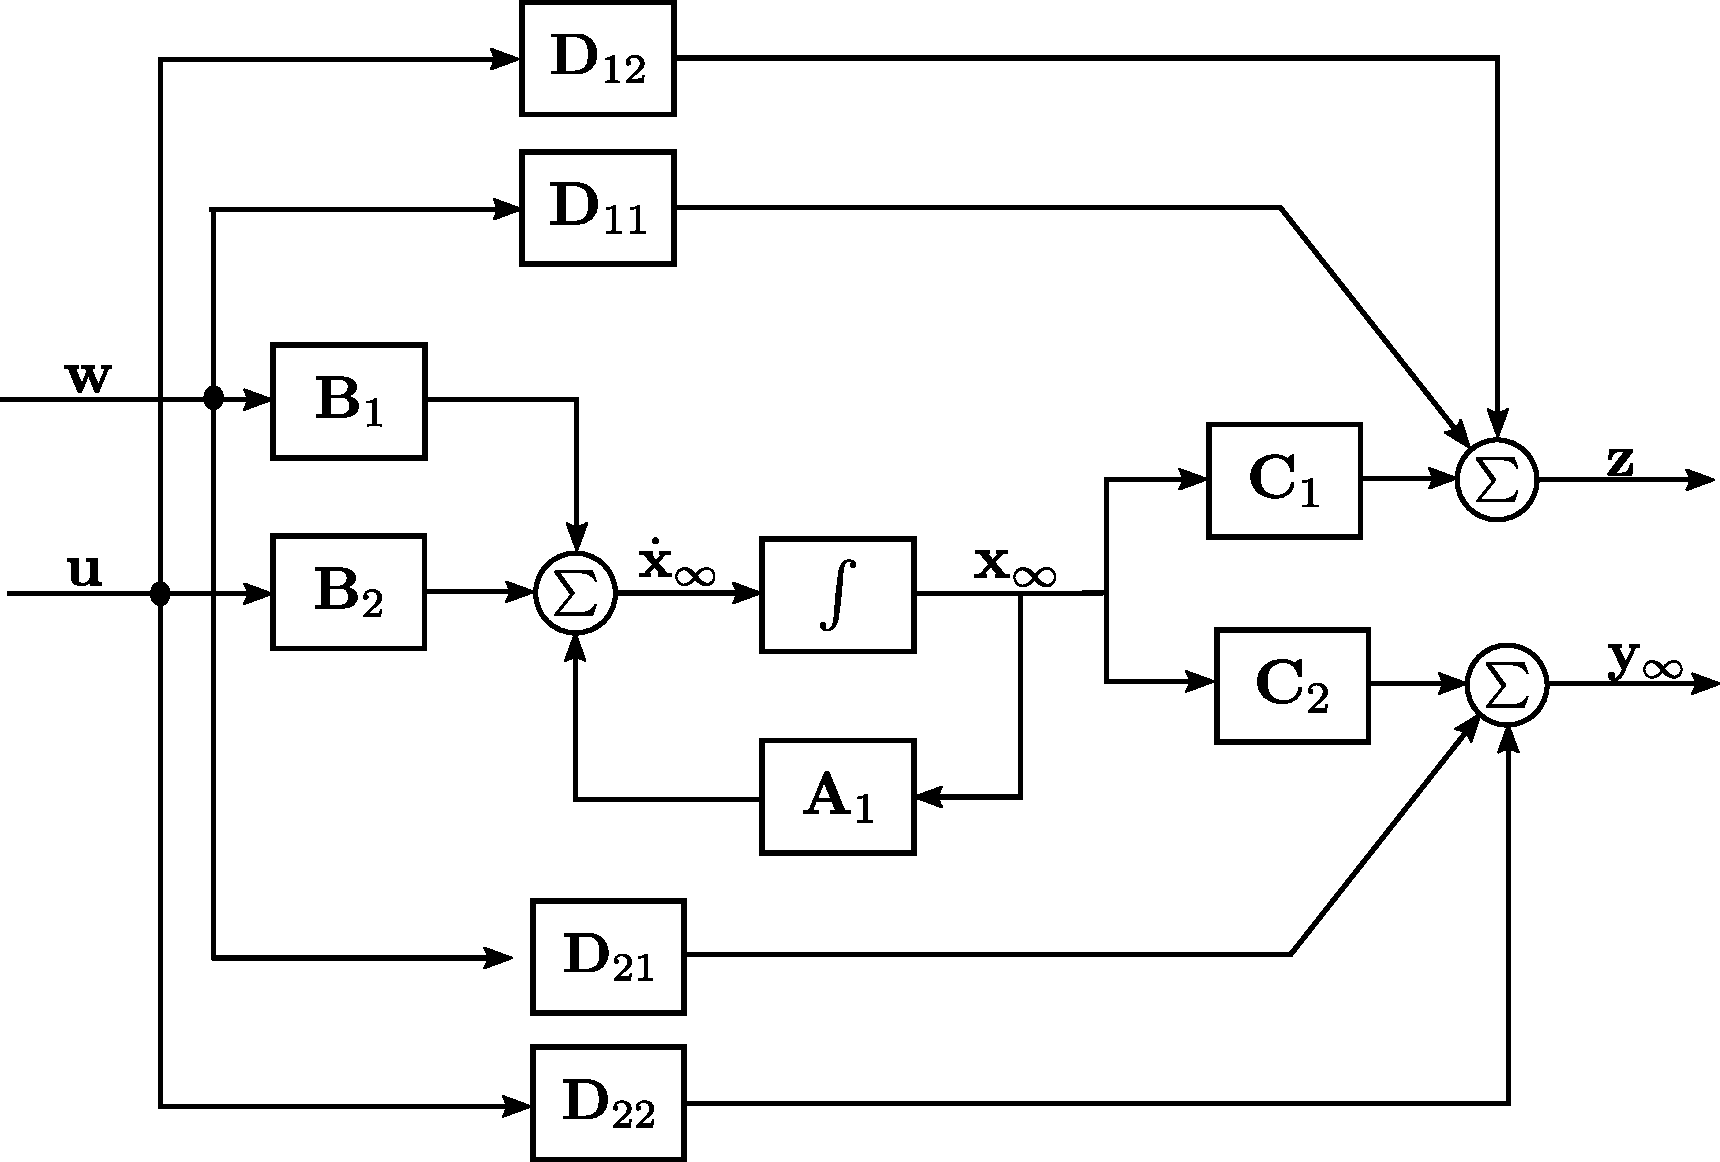
\includegraphics[width=0.55\linewidth]{figures/HinfDiag}
    \end{figure}
    \begin{minipage}[t][2.5cm]{\textwidth}
        \begin{flalign}	
        \vec{z}(t) &= 
        \begin{bmatrix}
        \vec{x}_\infty^\mathrm{T} & \vec{u}^\mathrm{T}
        \end{bmatrix}^\mathrm{T}\nonumber		
        \end{flalign}
    \end{minipage}
\end{frame}

\begin{frame}{Inner Controller}{$\mathcal{H}_\infty$ Controller Design}
    \begin{itemize}
        \item Controller design parameters ($\gamma$, $\vec{C}_1$, $\vec{D}_{12}$)
    \end{itemize}  
    \begin{minipage}{0.65\linewidth}
        \begin{flalign}
        \vec{C}_1 &=
        \begin{bmatrix}
            \vec{W}_\mathrm{x} & \vec{0}_{3\mathrm{x}2} &  \vec{0}_{3\mathrm{x}2} &  \vec{0}_{3\mathrm{x}2}  & \vec{0}_{3\mathrm{x}2} \\
            \vec{0}_{2\mathrm{x}3}  &  \vec{W}_\mathrm{I}  & \vec{0}_{2\mathrm{x}2} &  \vec{0}_{2\mathrm{x}2}  & \vec{0}_{2\mathrm{x}2} \\
            \vec{0}_{2\mathrm{x}3}  & \vec{0}_{2\mathrm{x}2} &  \vec{W}_\mathrm{wc} &  \vec{0}_{2\mathrm{x}2} &  \vec{0}_{2\mathrm{x}2} \\
            \vec{0}_{2\mathrm{x}3} &  \vec{0}_{2\mathrm{x}2}  & \vec{0}_{2\mathrm{x}2}  & \vec{W}_\mathrm{wave}  & \vec{0}_{2\mathrm{x}2} \\
            \vec{0}_{2\mathrm{x}3} &  \vec{0}_{2\mathrm{x}2}  & \vec{0}_{2\mathrm{x}2} &  \vec{0}_{2\mathrm{x}2} &  \vec{W}_\mathrm{noise} \\
            \vec{0}_{2\mathrm{x}3}  & \vec{0}_{2\mathrm{x}2}  & \vec{0}_{2\mathrm{x}2}  & \vec{0}_{2\mathrm{x}2} &  \vec{0}_{2\mathrm{x}2} \\
            \vec{0}_{2\mathrm{x}3}  & \vec{0}_{2\mathrm{x}2}  & \vec{0}_{2\mathrm{x}2}  & \vec{0}_{2\mathrm{x}2}  & \vec{0}_{2\mathrm{x}2} 
        \end{bmatrix}\nonumber
        \end{flalign} 
    \end{minipage}\hfill  
    \begin{minipage}{0.3\linewidth}
        \begin{flalign}
            \vec{D}_{12} &=
            \begin{bmatrix}
                \vec{0}_{2\mathrm{x}3} \\
                \vec{0}_{2\mathrm{x}2} \\
                \vec{0}_{2\mathrm{x}2} \\
                \vec{0}_{2\mathrm{x}2} \\
                \vec{0}_{2\mathrm{x}2} \\
                \vec{W}_\mathrm{u}
            \end{bmatrix} \nonumber
        \end{flalign}
    \end{minipage}\hfill 
 
\end{frame}


\begin{frame}{Inner Controller}{$\mathcal{H}_\infty$ Controller Design}
    \begin{itemize}
        \item Feedback gain
    \end{itemize}
    \begin{flalign}
        \vec{X}_\infty = Ric
        \begin{bmatrix}
        \vec{A}_1 & \gamma^{-2}\vec{B}_1\vec{B}_1^\mathrm{T} - \vec{B}_2\vec{B}_2^\mathrm{T} \\
        -\vec{C}_1^\mathrm{T}\vec{C}_1 & -\vec{A}_1^\mathrm{T}
        \end{bmatrix} \nonumber
    \end{flalign}
    \begin{flalign}
        \vec{F}_\infty = -\vec{B}_2^\mathrm{T}\vec{X}_\infty \nonumber
    \end{flalign}
\end{frame}


\definecolor{aaublue}{RGB}{33,26,82}% dark blue

\begin{frame}<handout:0>{Agenda}{}
    \begin{itemize}
        \item Introduction
        \item System Description
        \item Model
        \item Control Approach
        \item Sensor Fusion
        \item \textcolor{aaublue}{\textbf{Inner Controller}}
        \begin{itemize}
            \item[-] $\mathcal{H}_\infty$ Controller Design
            \item[-] \textcolor{aaublue}{\textbf{Linear Quadratic Regulator Design}}
            \item[-] \textcolor{aaublue}{\textbf{Controllers Comparison}}
        \end{itemize}
        \item Outer Controller
        \item Results
        \item Conclusion
    \end{itemize}
\end{frame}
\begin{frame}{Inner Controller}{Linear Quadratic Controller Design}

\only<1| handout:0>
{
  %\item Discrete system representation

  \tikz[overlay,xshift=15em,yshift=1em]{\draw node {
      \begin{minipage}{1\linewidth}
        \begin{figure}[H]
          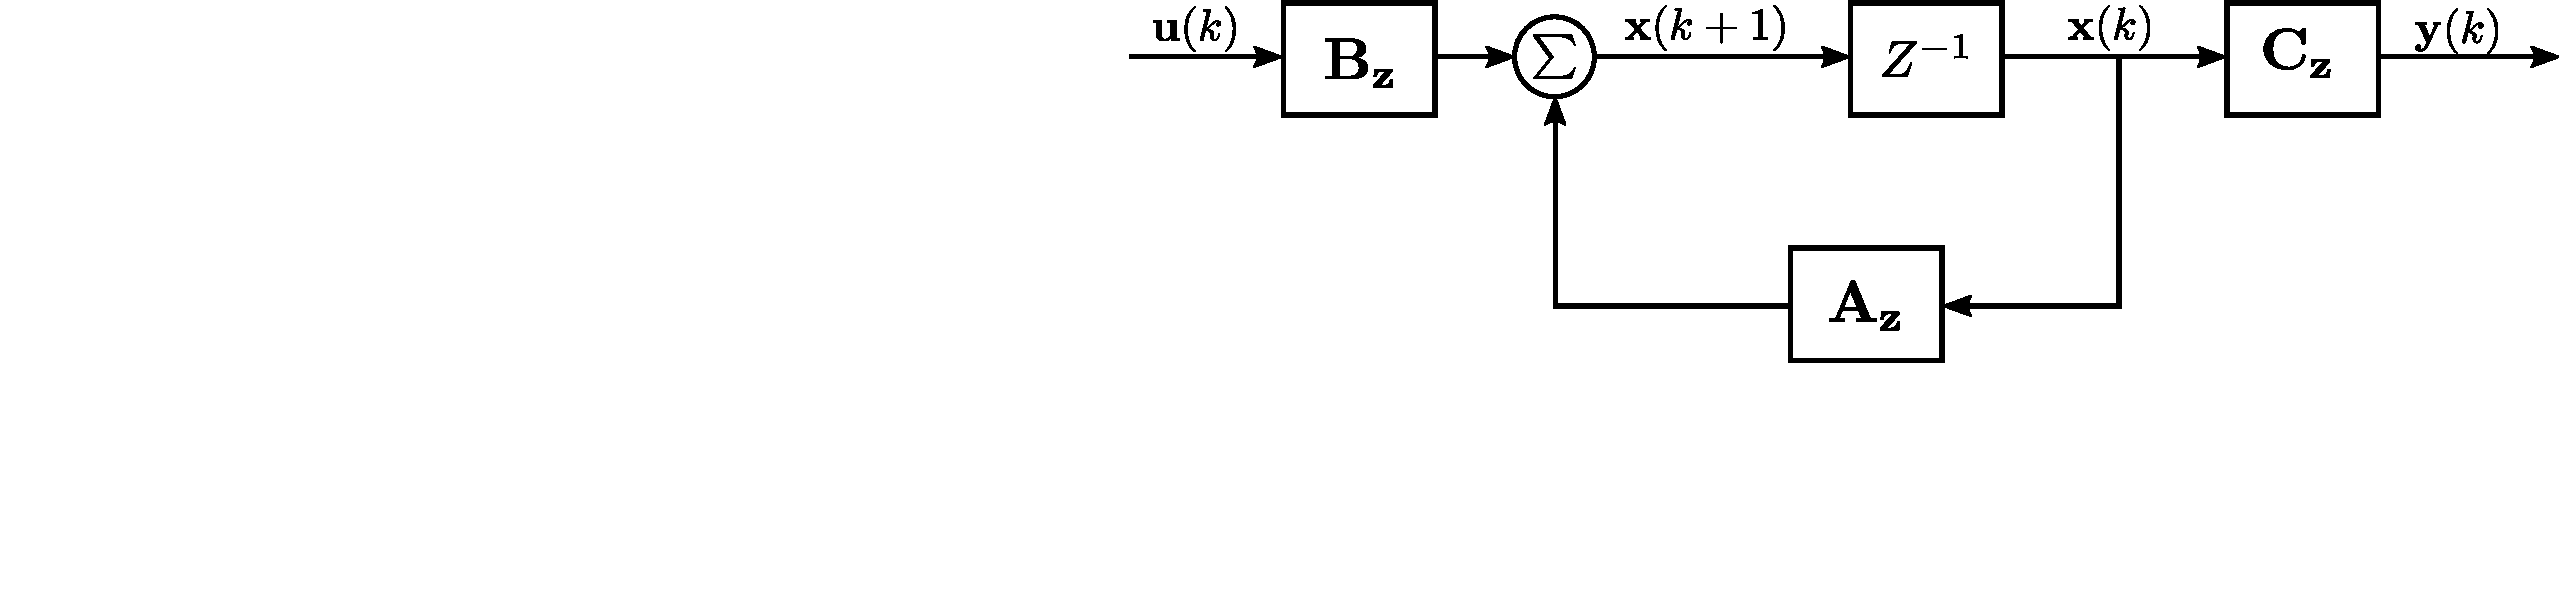
\includegraphics[width=1\textwidth]{figures/LQRblockDiagram1}
        \end{figure}
      \end{minipage}
    };}
  
  
  \tikz[overlay,xshift=12em,yshift=-5em]{\draw node {
      \begin{minipage}{0.01\linewidth}
        \begin{flalign}
          \vec{x}(k+1) &= \vec{A}_z  \vec{x}(k) + \vec{B}_z  \vec{u}(k) \nonumber \\
          \vec{y}(k) &= \vec{C}_z x(k) + \vec{D}_z  \vec{u}(k) \nonumber
        \end{flalign}
      \end{minipage}
  };}
  
}

\only<2-4| handout:1>
{
  %\item Adding a reference
  \tikz[overlay,xshift=15em,yshift=1em]{\draw node {
    \begin{minipage}{1\linewidth}
      \begin{figure}[H]
        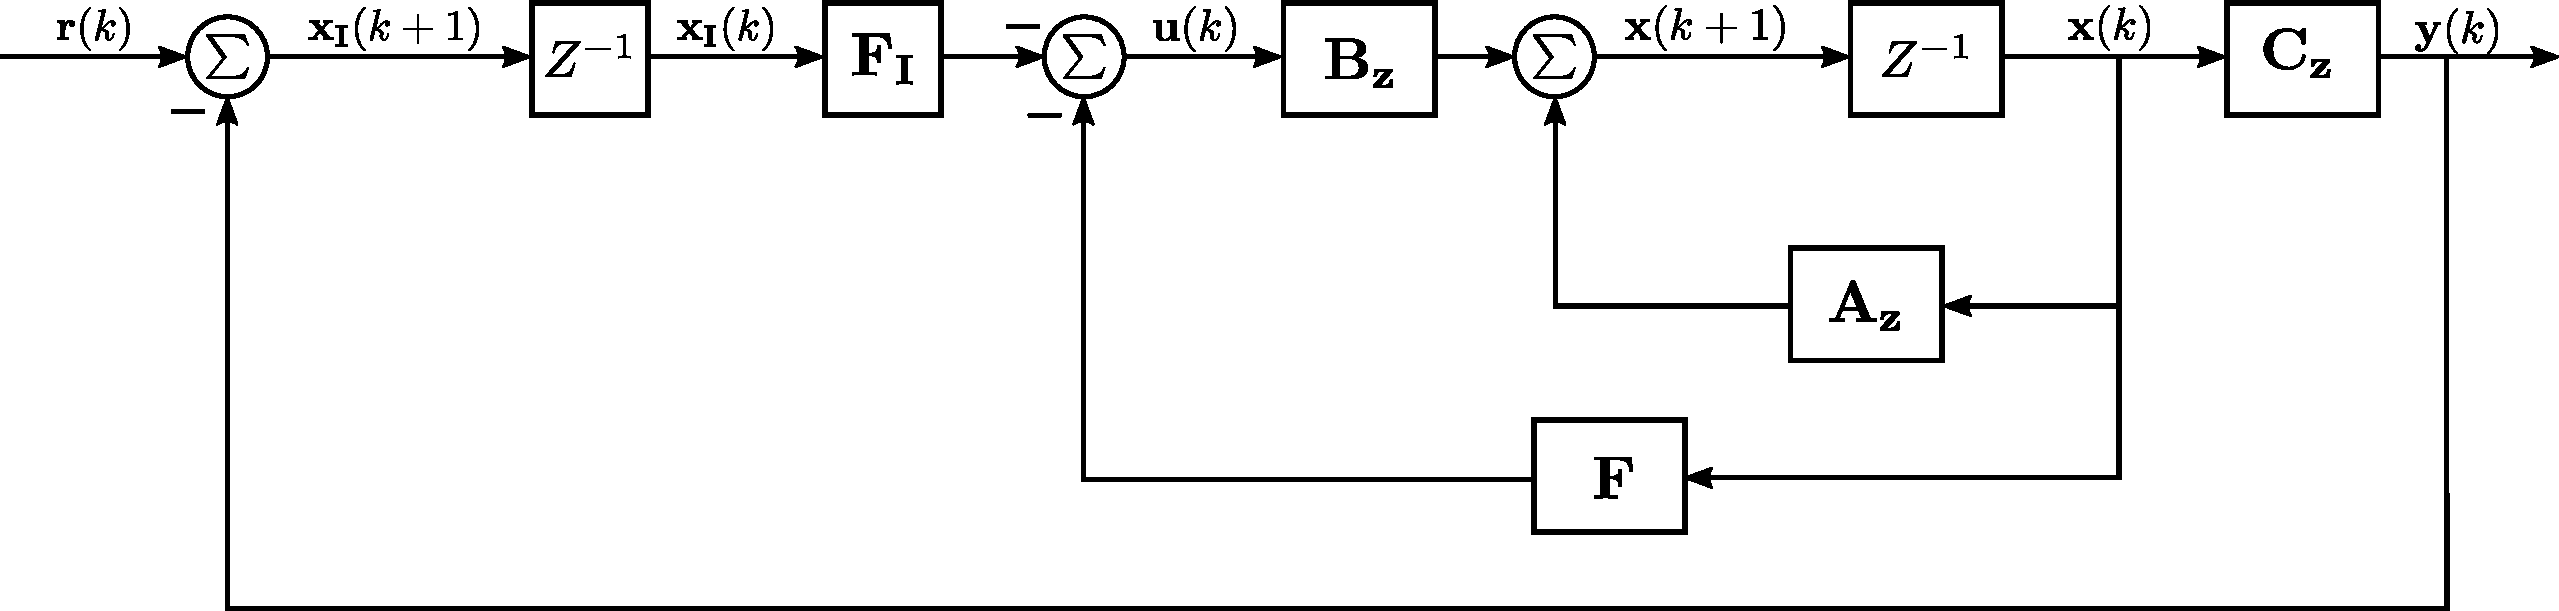
\includegraphics[width=1\textwidth]{figures/LQRblockDiagram2}
      \end{figure}
    \end{minipage}
  };}
}

%\only<0| handout:1>
%{
%  \tikz[overlay,xshift=12em,yshift=-2.5em]{\draw node {
%      \begin{minipage}{0.01\linewidth}
%        \begin{flalign}
%        \vec{x}(k+1) &= \vec{A}_z  \vec{x}(k) + \vec{B}_z  \vec{u}(k) \nonumber \\
%        \vec{y}(k) &= \vec{C}_z x(k) + \vec{D}_z  \vec{u}(k) \nonumber
%        \end{flalign}
%      \end{minipage}
%    };}
%}

\only<2| handout:0>
{
  \tikz[overlay,xshift=12em,yshift=-5.5em]{\draw node {
  };}
}

\only<3| handout:0>
{
  \tikz[overlay,xshift=12em,yshift=-5em]{\draw node {
    \begin{minipage}{0.01\linewidth}
      \begin{flalign}
        \vec{x}_e(k+1) &= \vec{A}_e  \vec{x}_e(k) + \vec{B}_e  \vec{u}(k) + \vec{r}(k) \nonumber \\
        \vec{y}(k) &= \vec{C}_e  \vec{x}_e(k) \nonumber
      \end{flalign}
    \end{minipage}
  };}
}

\only<4| handout:1>
{
  \tikz[overlay,xshift=12em,yshift=-5.5em]{\draw node {
    \begin{minipage}{0.01\linewidth}
      \begin{flalign}
      \hspace{2cm}
        \begin{bmatrix}
          \vec{x}(k+1)  \\
          \vec{x}_\mathrm{I}(k+1)
        \end{bmatrix}
        &=
        \begin{bmatrix}
         \ \ \ \vec{A}_\mathrm{z,3x3} & \vec{0}_\mathrm{3x2} \\
         -\vec{C}_\mathrm{z,2x3} & \vec{I}_\mathrm{2x2} \\
        \end{bmatrix}
        \begin{bmatrix}
          \vec{x}(k)    \\
          \vec{x}_\mathrm{I}(k)
        \end{bmatrix}
        +
        \begin{bmatrix}
          \vec{B}_\mathrm{z,3x2} \\
          \vec{0}_\mathrm{2x2}
        \end{bmatrix}
        \vec{u}(k)
        +
        \begin{bmatrix}
          \vec{0}_\mathrm{3x2} \\
          \vec{I}_\mathrm{2x2}
        \end{bmatrix}
        \vec{r}(k) \nonumber \\ \nonumber \\[-10pt]
        \vec{y}(k)
        &=
        \begin{bmatrix}
          \vec{C}_\mathrm{z,2x3} &  \vec{0}_\mathrm{2x2}
        \end{bmatrix}
        \begin{bmatrix}
          \vec{x}(k)    \\
          \vec{x}_\mathrm{I}(k)
        \end{bmatrix} \nonumber
      \end{flalign}
    \end{minipage}
  };}
}

\end{frame}



\begin{frame}{Inner Controller}{Linear Quadratic Controller Design}

\only<1| handout:0>
{
  \tikz[overlay,xshift=12em,yshift=5.5em]{\draw node {
    \begin{minipage}{0.01\linewidth}
      \begin{flalign}
      \mathcal{J}_\mathrm{z} = \sum_{k=0}^\infty \vec{x}^\mathrm{T}(k)\vec{Q}_\mathrm{z}\vec{x}(k) + \vec{u}^\mathrm{T}(k)\vec{R}_\mathrm{z}\vec{u}(k) \nonumber
      \end{flalign}
    \end{minipage}
  };}
  \tikz[overlay,xshift=12em,yshift=1em]{\draw node {
  };}
  \tikz[overlay,xshift=12em,yshift=-5em]{\draw node {
  };}
}

\only<2-4| handout:1>
{
  \tikz[overlay,xshift=12em,yshift=5.5em]{\draw node {
      \begin{minipage}{0.01\linewidth}
        \begin{flalign}
        \mathcal{J}= \int_{0}^\infty \vec{x}^\mathrm{T}(t)\vec{Q}\vec{x}(t) + \vec{u}^\mathrm{T}(t)\vec{R}\vec{u}(t) \ dt \nonumber
        \end{flalign}
      \end{minipage}
    };}
  \tikz[overlay,xshift=12em,yshift=1em]{\draw node {
    };}
  \tikz[overlay,xshift=12em,yshift=-5em]{\draw node {
    };}
}


\only<1-2| handout:0>
{
  \tikz[overlay,xshift=12em,yshift=1em]{\draw node {
  };}
}

\only<3-4| handout:1>
{
  \tikz[overlay,xshift=12em,yshift=1em]{\draw node {
    \begin{minipage}{0.01\linewidth}
      \begin{flalign} 
        \hspace{2cm}
        Q &= \left(
        \frac{1}{{\psi_\mathrm{max}}\text{}^2} \ , \ 
        \frac{1}{{\dot{\psi}_\mathrm{max}}\text{}^2} \ , \ 
        \frac{1}{{\dot{x}_{b,\mathrm{max}}}\text{}^2} \ , \ 
        \frac{1}{x_{\mathrm{I},\psi,\mathrm{max}}\text{}^2} \ , \ 
        \frac{1}{x_{\mathrm{I},\dot{\psi},\mathrm{max}}\text{}^2} \ , \ 
        \frac{1}{x_{\mathrm{I},\dot{x_b},\mathrm{max}}\text{}^2} \right)
        \nonumber
      \end{flalign}
%      \begin{flalign}
%      \dot{\vec{x}}(t) &= \vec{A}  \vec{x}(t) + \vec{B}  \vec{u}(t) + r(t)\nonumber \\
%      \vec{y}(t) &= \vec{C} x(t)  \nonumber
%      \end{flalign}
    \end{minipage}
  };}
}

\only<1-3| handout:0>
{
  \tikz[overlay,xshift=12em,yshift=-5em]{\draw node {
  };}
}

\only<4| handout:1>
{
  \tikz[overlay,xshift=12em,yshift=-5em]{\draw node {
  \begin{minipage}{0.01\linewidth}
    \begin{flalign}
      \hspace{2cm}
      R &= \left(
      \frac{1}{{{F_1}_\mathrm{max}}\text{}^2} \ , \ 
      \frac{1}{{{F_2}_\mathrm{max}}\text{}^2} \right)
      \nonumber
    \end{flalign}
%    \begin{flalign}
%      \hspace{2cm}
%      \begin{bmatrix}
%        \dot{\vec{x}}(t)  \\
%        \dot{\vec{x}}_\mathrm{I}(t)
%      \end{bmatrix}
%      &=
%      \begin{bmatrix}
%      \ \ \ \vec{A}_\mathrm{3x3} & \vec{0}_\mathrm{3x2} \\
%       -\vec{C}_\mathrm{2x3} & \vec{I}_\mathrm{2x2} \\
%      \end{bmatrix}
%      \begin{bmatrix}
%        \vec{x}(t)    \\
%        \vec{x}_\mathrm{I}(t)
%      \end{bmatrix}
%      +
%      \begin{bmatrix}
%        \vec{B}_\mathrm{3x2} \\
%        \vec{0}_\mathrm{2x2}
%      \end{bmatrix}
%      \vec{u}(k)
%      +
%      \begin{bmatrix}
%        \vec{0}_\mathrm{3x2} \\
%        \vec{I}_\mathrm{2x2}
%      \end{bmatrix}
%      \vec{r}(t) \nonumber \\ \nonumber \\[-10pt]
%      \vec{y}(t)
%      &=
%      \begin{bmatrix}
%        \vec{C}_\mathrm{2x3} &  \vec{0}_\mathrm{2x2}
%      \end{bmatrix}
%      \begin{bmatrix}
%        \vec{x}(t)    \\
%        \vec{x}_\mathrm{I}(t)
%      \end{bmatrix} \nonumber
%    \end{flalign}
  \end{minipage}
  };}
}
\end{frame}



\begin{frame}{Inner Controller}{Comparison of the Controllers}
  Simulation of LQR and robust design
  \begin{itemize}
    \item<1-> Disturbances from wind and waves
    \begin{itemize}
      \item<1-> $\pm 1.5$ N along $\dot{x}_b$
      \item<1-> $\pm 1.5$ N$\cdot$m around $z_b$
      \item<1-> The frequency for both varies between $0$-$10$ Hz 
    \end{itemize}
    \item<2-> The parameters are varied $\pm 20\%$
    \begin{itemize}
      \item<2-> Mass, $m$
      \item<2-> Moment of inertia, $I_z$, around $z_b$
      \item<2-> The damping coefficients $d_x$ and $d_\psi$
      \item<2-> The lengths $l_1$ and $l_2$
    \end{itemize}
  \item<3-> Monte Carlo simulations with $1000$ realizations
  \end{itemize}
\end{frame}


\begin{frame}{Inner Controller}{Comparison of the Controllers}
\begin{figure}[H]
  \begin{minipage}{0.45\linewidth}
    \begin{figure}[H]
      \centering
      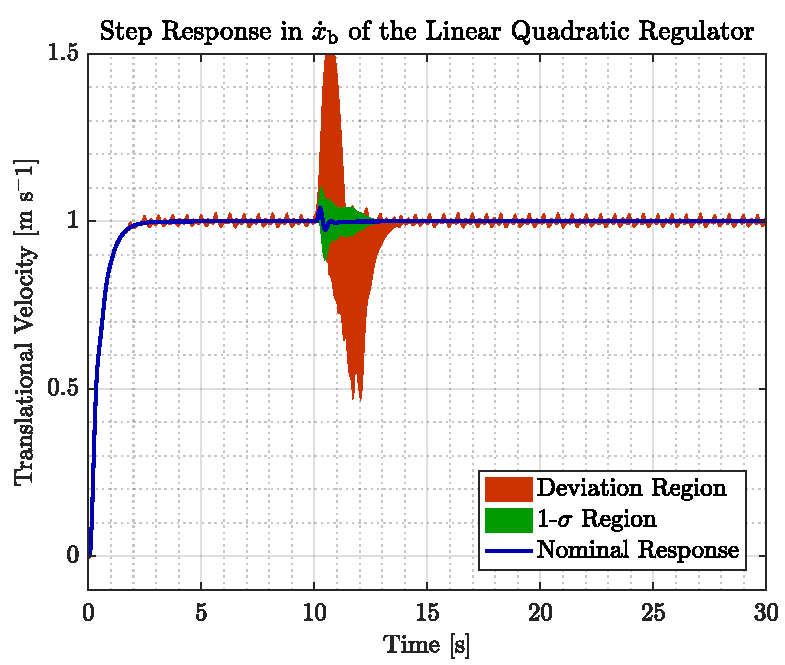
\includegraphics[width=1\linewidth]{figures/xbdot_mc_lqr}
    \end{figure}        
  \end{minipage}\hfill      
  \begin{minipage}{0.45\linewidth}
    \begin{figure}[H]
      \centering
      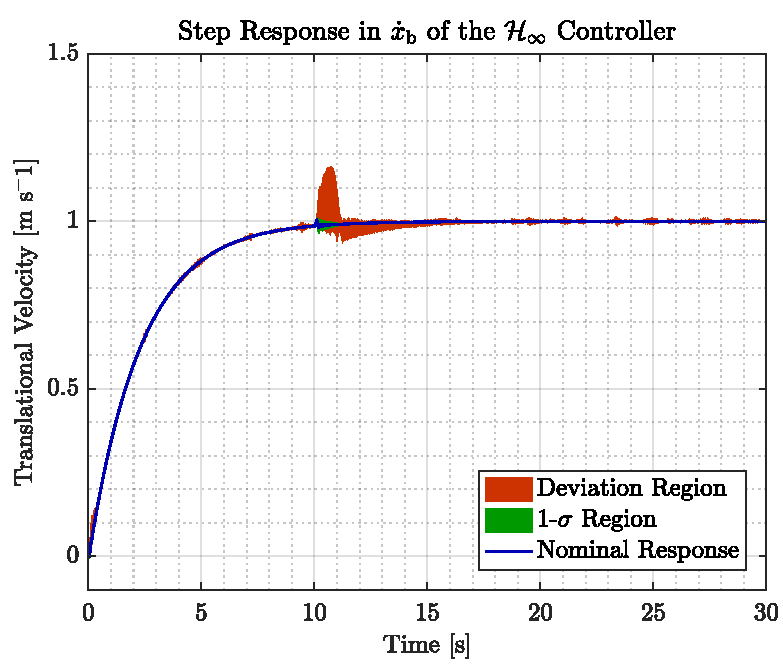
\includegraphics[width=1\linewidth]{figures/xbdot_mc_rob}
    \end{figure}                
  \end{minipage}\hfill \\
\end{figure}
\end{frame}



\begin{frame}{Inner Controller}{Comparison of the Controllers}
  \begin{figure}[H]
    \begin{minipage}{0.45\linewidth}
      \begin{figure}[H]
        \centering
        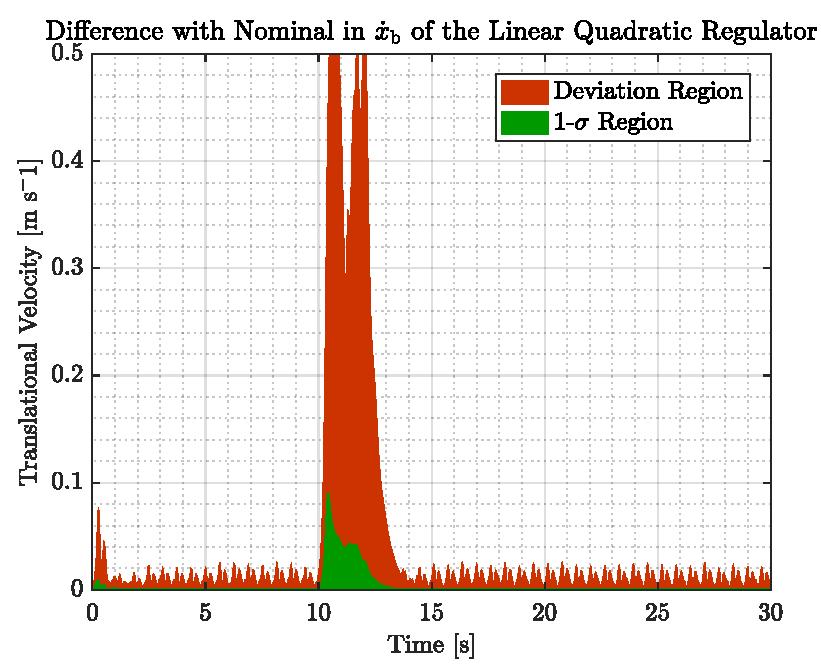
\includegraphics[width=1\linewidth]{figures/xbdot_mc_lqr_error}
      \end{figure}        
    \end{minipage}\hfill      
    \begin{minipage}{0.45\linewidth}
      \begin{figure}[H]
        \centering
        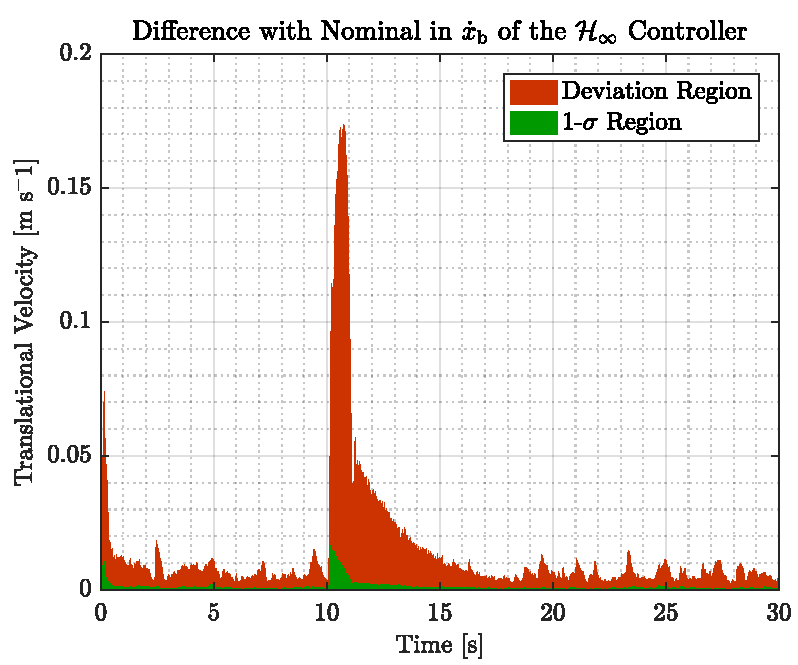
\includegraphics[width=1\linewidth]{figures/xbdot_mc_rob_error}
      \end{figure}                
    \end{minipage}\hfill \\
  \end{figure}
\end{frame}



\begin{frame}{Inner Controller}{Comparison of the Controllers}
  \begin{figure}[H]
    \begin{minipage}{0.45\linewidth}
      \begin{figure}[H]
        \centering
        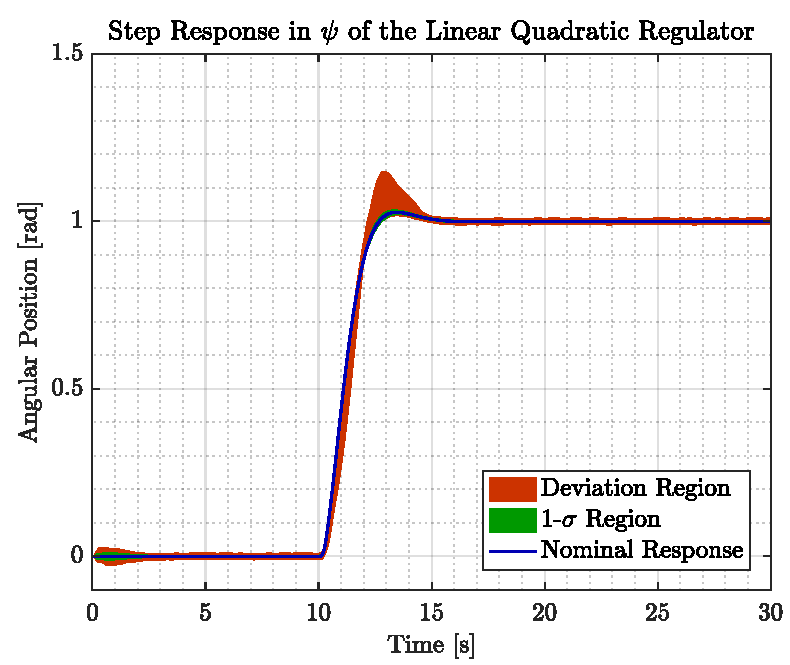
\includegraphics[width=1\linewidth]{figures/yaw_mc_lqr}
      \end{figure}        
    \end{minipage}\hfill      
    \begin{minipage}{0.45\linewidth}
      \begin{figure}[H]
        \centering
        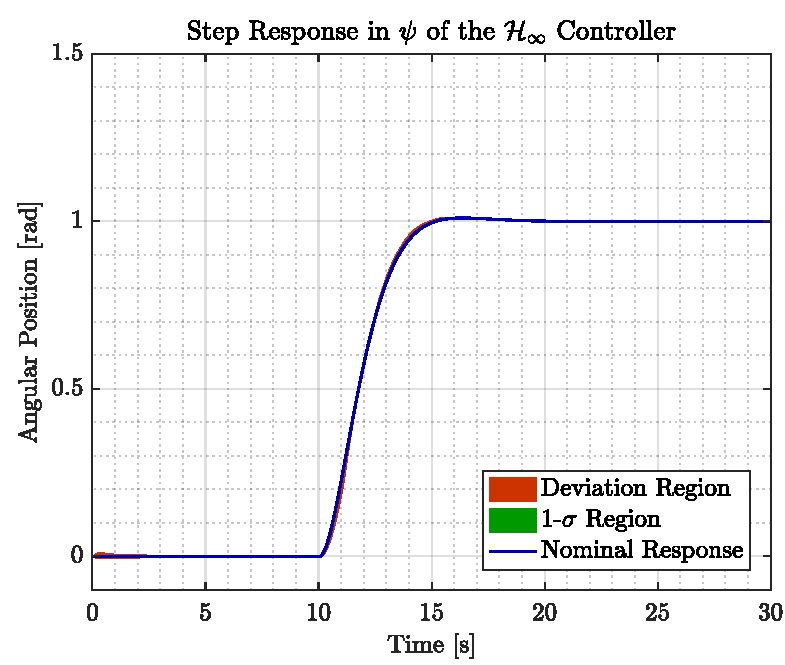
\includegraphics[width=1\linewidth]{figures/yaw_mc_rob}
      \end{figure}                
    \end{minipage}\hfill \\
  \end{figure}
\end{frame}



\begin{frame}{Inner Controller}{Comparison of the Controllers}
  \begin{figure}[H]
    \begin{minipage}{0.45\linewidth}
      \begin{figure}[H]
        \centering
        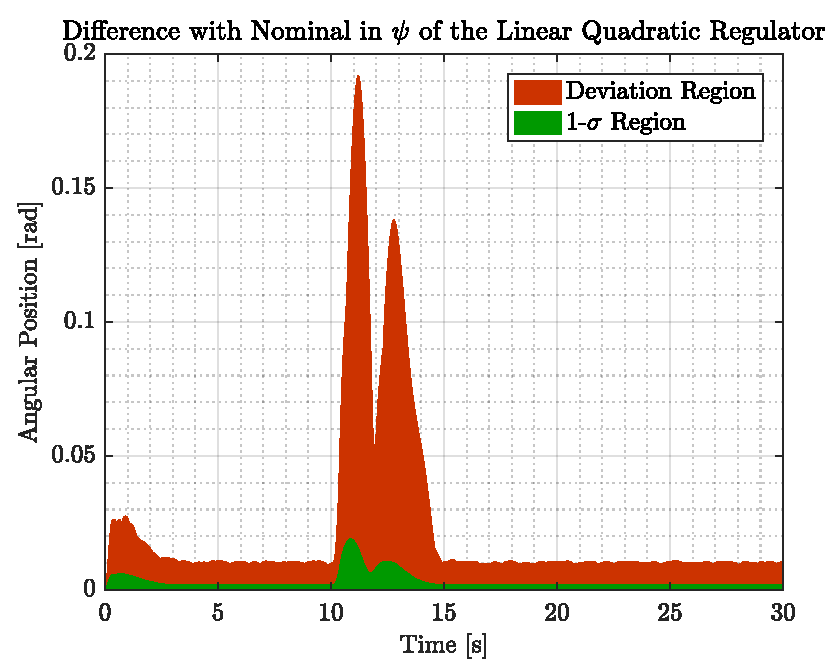
\includegraphics[width=1\linewidth]{figures/yaw_mc_lqr_error}
      \end{figure}        
    \end{minipage}\hfill      
    \begin{minipage}{0.45\linewidth}
      \begin{figure}[H]
        \centering
        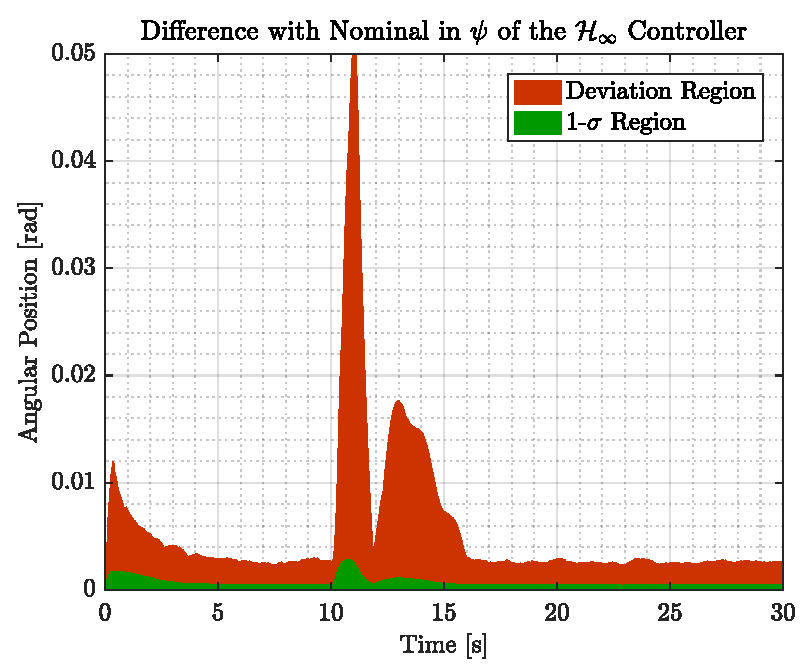
\includegraphics[width=1\linewidth]{figures/yaw_mc_rob_error}
      \end{figure}                
    \end{minipage}\hfill \\
  \end{figure}
\end{frame}



\begin{frame}{Agenda}{}
    \begin{itemize}
        \item Introduction
        \item System Description
        \item Model
        \item Control Approach
        \item Sensor Fusion
        \item Inner Controller
        \item \textbf{Outer Controller}
        \begin{itemize}
            \item[-] \textbf{Path Generation Algorithm}
            \item[-] \textbf{Path Following Algorithm}
        \end{itemize}
        \item \textbf{Results}
        \begin{itemize}
            \item[-] \textbf{Controller Results}
            \item[-] \textbf{Implementation Results}
        \end{itemize}
        \item \textbf{Conclusion}
    \end{itemize}
\end{frame}
%%%%%%%%%%%%%%%%
\section{Outer Controller}

\begin{frame}{Outer Controller}{Path Generation Algorithm}
    \begin{figure}[H]
        \centering
        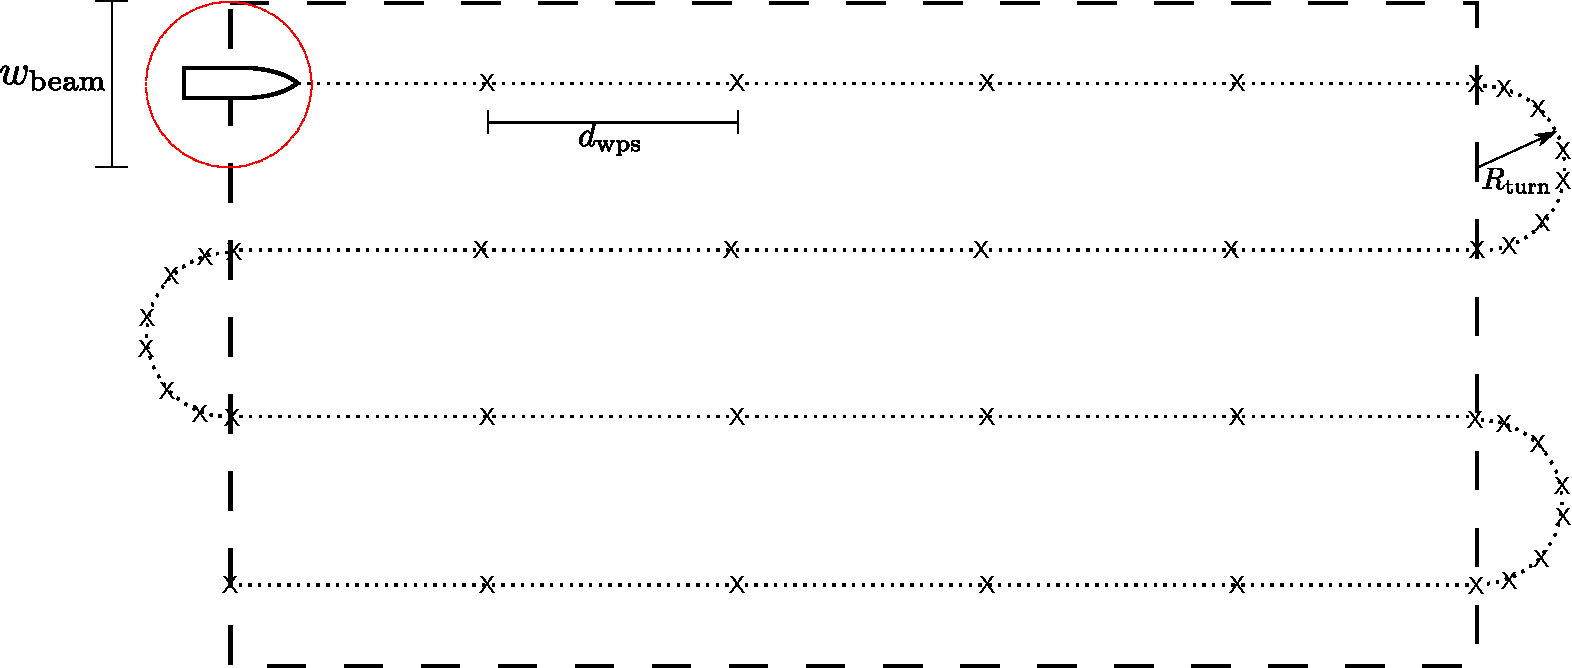
\includegraphics[width=1\textwidth]{figures/pathGen} 
    \end{figure}       
\end{frame}

\begin{frame}{Outer Controller}{Path Following Algorithm}
    \begin{minipage}{0.6\linewidth}
        \uncover<1-4>{
        \begin{figure}[H]
            \centering
            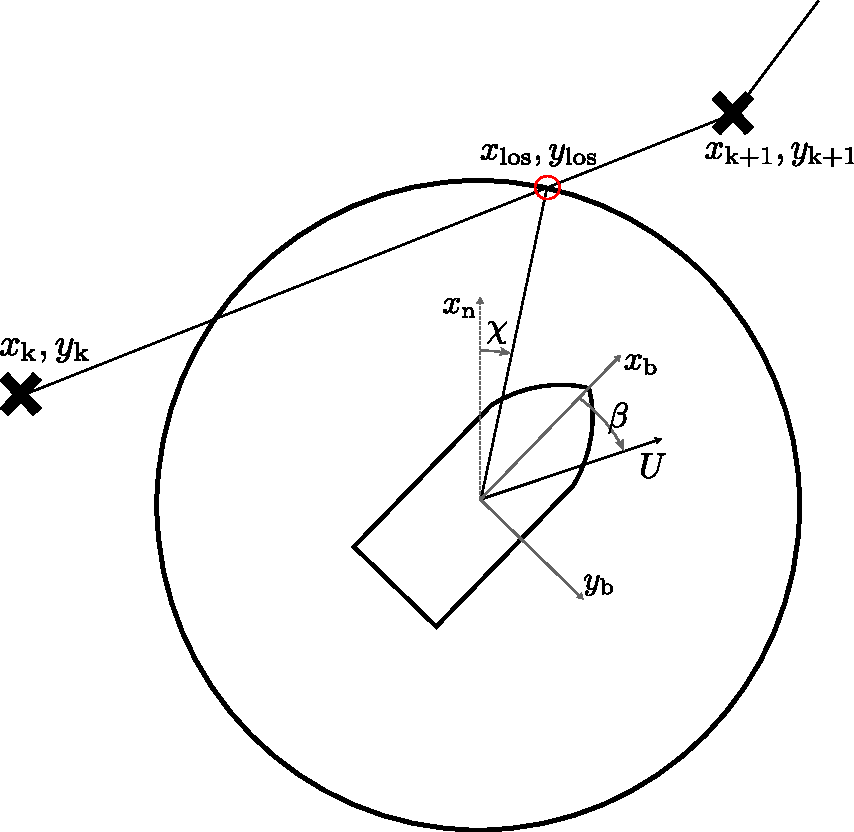
\includegraphics[width=0.9\linewidth]{figures/LOSalgorithm}
        \end{figure} }       
    \end{minipage}\hfill      
    \begin{minipage}{0.2\linewidth}
        \uncover<2-4>{
        \begin{flalign}
            \chi &= \arctan\left(\frac{y_\mathrm{LOS}-y_\mathrm{n}}{x_\mathrm{LOS}-x_\mathrm{n}}\right)\nonumber 
        \end{flalign} }
        \uncover<3-4>{
        \begin{flalign}
            \beta &= \arctan\left(\frac{\dot{y}_\mathrm{b}}{\dot{x}_\mathrm{b}}\right) \nonumber
        \end{flalign} }
        \uncover<4>{
        \begin{flalign}
            \psi&_\mathrm{ref} = \chi - \beta \nonumber
        \end{flalign}}          
    \end{minipage}\hfill \\ 
\end{frame}

\begin{frame}{Outer Controller}{Path Following Algorithm}
    \begin{itemize}
        \item Change active waypoints
    \end{itemize}
    \begin{figure}[H]
        \centering
        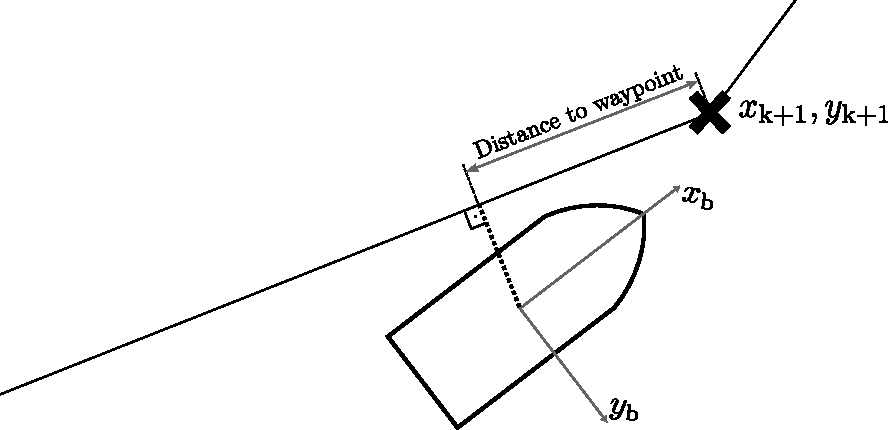
\includegraphics[width=0.6\linewidth]{figures/LOSalgorithmdistancewp}
    \end{figure}
\end{frame}
\begin{frame}{Outer Controller}{Path Following Algorithm}
    \begin{itemize}
        \item Convergence to the path
    \end{itemize}
    \begin{minipage}{0.45\linewidth}
        \begin{figure}[H]
            \centering
            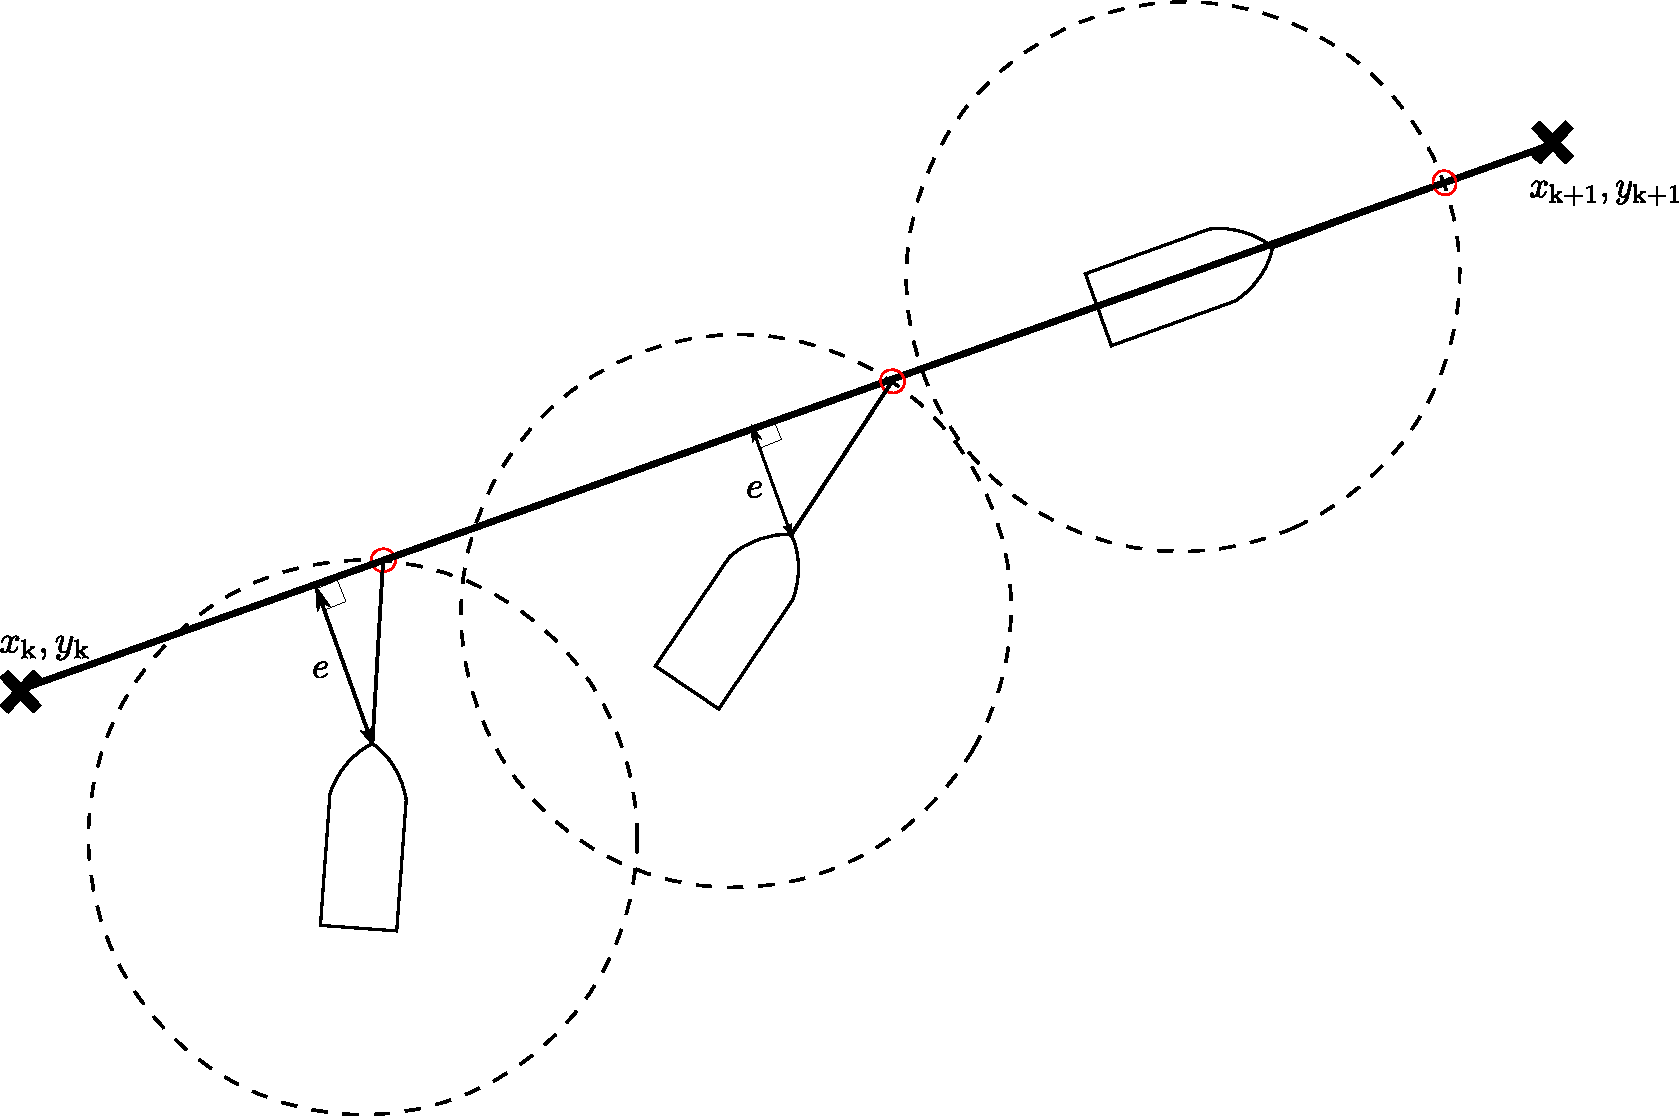
\includegraphics[width=1\linewidth]{figures/patherror}
        \end{figure}     
    \end{minipage}\hfill      
    \begin{minipage}{0.45\linewidth}
        \begin{figure}[H]
            \centering
            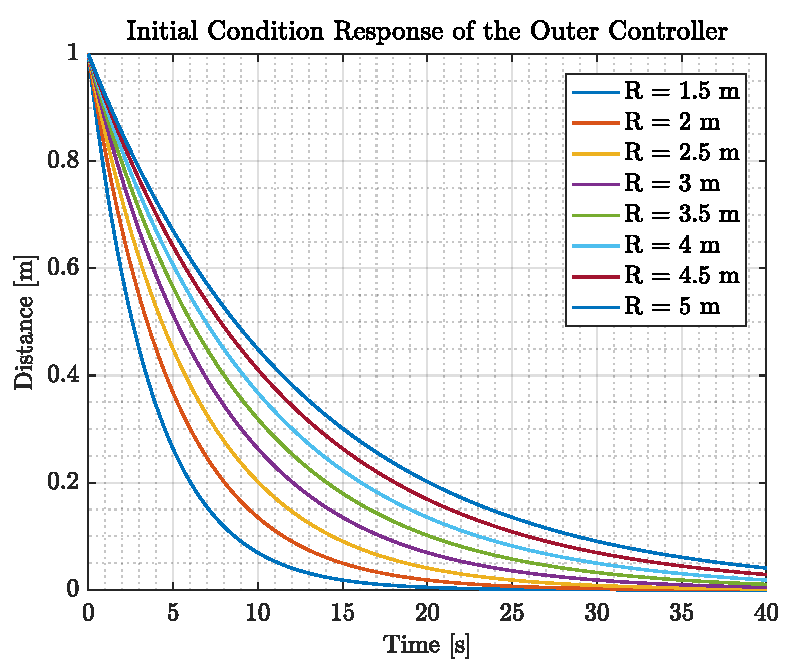
\includegraphics[width=1\linewidth]{figures/initCondOuter}
        \end{figure}               
    \end{minipage}\hfill \\
\end{frame}
%%%%%%%%%%%%%%%%
\section{Results}

\begin{frame}{Results}{Controller Results}
\begin{itemize}
    \item LQR as inner controller
\end{itemize}
    \begin{minipage}{0.45\linewidth}
            \begin{figure}[H]
                \centering
                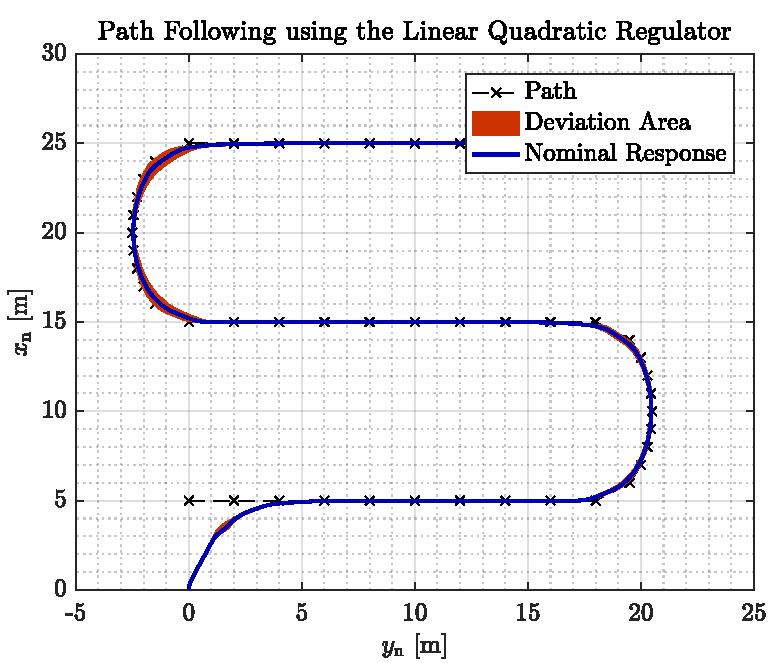
\includegraphics[width=1\linewidth]{figures/path_lqr}
            \end{figure}        
        \end{minipage}\hfill      
    \begin{minipage}{0.45\linewidth}
            \begin{figure}[H]
                \centering
                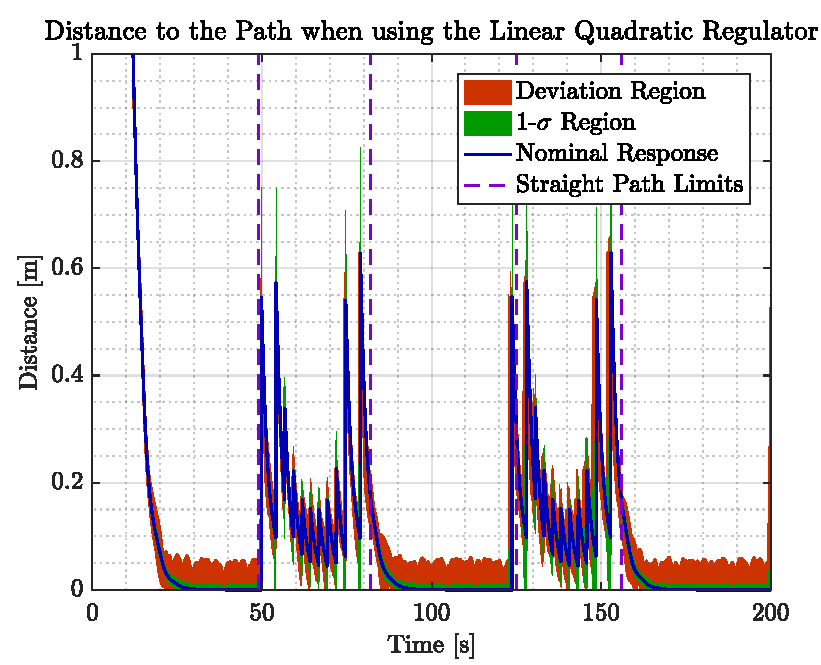
\includegraphics[width=1\linewidth]{figures/dist_lqr}
            \end{figure}               
        \end{minipage}\hfill \\    
\end{frame}

\begin{frame}{Results}{Controller Results}
    \begin{itemize}
        \item Robust controller as inner controller
    \end{itemize}
    \begin{minipage}{0.45\linewidth}
            \begin{figure}[H]
                \centering
                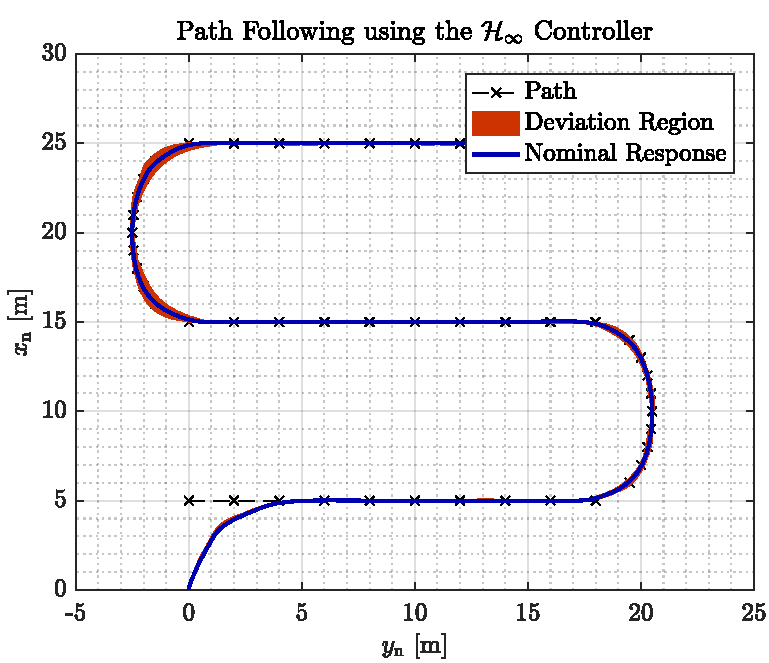
\includegraphics[width=1\linewidth]{figures/path_rob}
            \end{figure}       
        \end{minipage}\hfill      
    \begin{minipage}{0.45\linewidth}
            \begin{figure}[H]
                \centering
                \includegraphics[width=1\linewidth]{figures/dist_rob}
            \end{figure}             
        \end{minipage}\hfill \\    
\end{frame}

\begin{frame}{Results}{Implementation Results}
    \begin{itemize}
        \item Implementation diagram in ROS
    \end{itemize}
    \begin{figure}[H]
        \centering
        \includegraphics[width=1\textwidth]{figures/diagramROS}
    \end{figure}  
\end{frame}


\begin{frame}{Results}{Implementation Results}
    \begin{itemize}
        \item Inner controller test
    \end{itemize}
    \begin{minipage}{0.45\linewidth}
        \begin{figure}[H]
            \centering
            \includegraphics[width=1\linewidth]{figures/inner_yaw}
        \end{figure}       
    \end{minipage}\hfill      
    \begin{minipage}{0.45\linewidth}
        \begin{figure}[H]
            \centering
            \includegraphics[width=1\linewidth]{figures/inner_xbdot}
        \end{figure}             
    \end{minipage}\hfill \\    
\end{frame}

\begin{frame}{Results}{Implementation Results}
    \begin{itemize}
        \item Actuator tests
    \end{itemize}
    \begin{minipage}{0.45\linewidth}
        \begin{figure}[H]
            \centering
            \includegraphics[width=1\linewidth]{figures/direction}
        \end{figure}       
    \end{minipage}\hfill      
    \begin{minipage}{0.45\linewidth}
        \begin{figure}[H]
            \centering
            \includegraphics[width=1\linewidth]{figures/hysteresis}
        \end{figure}             
    \end{minipage}\hfill \\    
\end{frame}

%%%%%%%%%%%%%%%%
\section{Conclusion}

\begin{frame}{Conclusion}{}
    \begin{itemize}
        \item The estimator has been tuned and tested through simulation.
    \end{itemize}
    \begin{itemize}
        \item The controller has also been analyzed though simulations that include disturbances, noise and varying parameters.
    \end{itemize}
    \begin{itemize}
        \item The simulated results have not been fully replicated in the real vessel, but they show a promising behavior of the control system.
    \end{itemize}
\end{frame}

%{\aauwavesbg
\begin{frame}[plain,noframenumbering]
    \finalpage{\large{Precision Control of an Autonomous Surface Vessel}}
\end{frame}%}

\end{document}
